\documentclass[12pt,a4paper,final]{book}
\usepackage[utf8]{inputenc}
\usepackage{graphicx}
\usepackage[italian]{babel}
\usepackage[a4paper, headheight=15mm, width=150mm,top=25mm,bottom=25mm,bindingoffset=6mm]{geometry}
\usepackage{fancyhdr}
\usepackage{xcolor}
\usepackage{cite}
\usepackage[final]{pdfpages}
\definecolor{codegreen}{rgb}{0,0.6,0}
\definecolor{codegray}{rgb}{0.5,0.5,0.5}
\definecolor{codepurple}{rgb}{0.58,0,0.82}
\definecolor{backcolour}{rgb}{0.95,0.95,0.92}
\usepackage{listings}
\lstdefinestyle{mystyle}{
    commentstyle=\color{codegreen},
    keywordstyle=\color{magenta},
    numberstyle=\tiny\color{codegray},
    stringstyle=\color{codepurple},
    basicstyle=\ttfamily\footnotesize,
    breakatwhitespace=false,
    breaklines=false,
    captionpos=b,
    keepspaces=true,
    numbers=left,
    numbersep=5pt,
    showspaces=false,
    showstringspaces=false,
    showtabs=false,
    tabsize=2
}
\lstset{style=mystyle}
\pagestyle{fancy}
\fancyhf{}
\fancyhead[L]{\nouppercase{\leftmark}}
\fancyhead[R]{\thepage}
\usepackage{amsmath}
\usepackage{mathtools}
\usepackage{nccmath}
\usepackage{mathrsfs}
\usepackage{subcaption}
\usepackage{afterpage}
\usepackage[pdfa]{hyperref}
%%%%%%%%%%%%%%%%%%%%%%%%%%%%%%%%%%%%%%%%%%%%%%%%%%%%%%%%
\title{Tesi di laurea triennale di Eleonora Gatti}
\author{Eleonora Gatti}
\date{Maggio/Luglio 2020}
%%%%%%%%%%%%%%%%%%%%%%%%%%%%%%%%%%%%%%%%%%%%%%%%%%%%%%%
%%%%%%%%%%%%%%%%%%%%%%%%%%%%%%%%%%%%%%%%%%%%%%%%%%%%%%%
%%%%%%%%%%%%%%%%%%%%%%%%%%%%%%%%%%%%%%%%%%%%%%%%%%%%%%%

\begin{document}

%%%%%%%%%%%%%%%%%%%%  PRIMA PAGINA  %%%%%%%%%%%%%%%%%%%


\includepdf[pages=-]{../frontespizio/frontespizio.pdf}
\newpage
\thispagestyle{empty}
\clearpage\mbox{}\clearpage
\newpage
\thispagestyle{empty}

%%%%%%%%%%%%%%%%%%%%%%%  INDICE  %%%%%%%%%%%%%%%%%%%%%

\tableofcontents
\newpage

%%%%%%%%%%%%%%%%%%%%  CAPITOLO 1  %%%%%%%%%%%%%%%%%%%%

\chapter{Sistemi ottici nelle microonde}\label{intro_sistemi_ottici}

    %%%%%%%%%%%%%%%%%%%  CAPITOLO 1.1  %%%%%%%%%%%%%%%%%%%

\section{Utilizzo delle microonde in astrofisica}\label{microonde_astrofisica}

    %%%%%%%%%%%%%%%%%%%  CAPITOLO 1.2  %%%%%%%%%%%%%%%%%%%

\section{Diagramma di radiazione}\label{rad_pattern}

\begin{figure}[!ht]
	\centering
	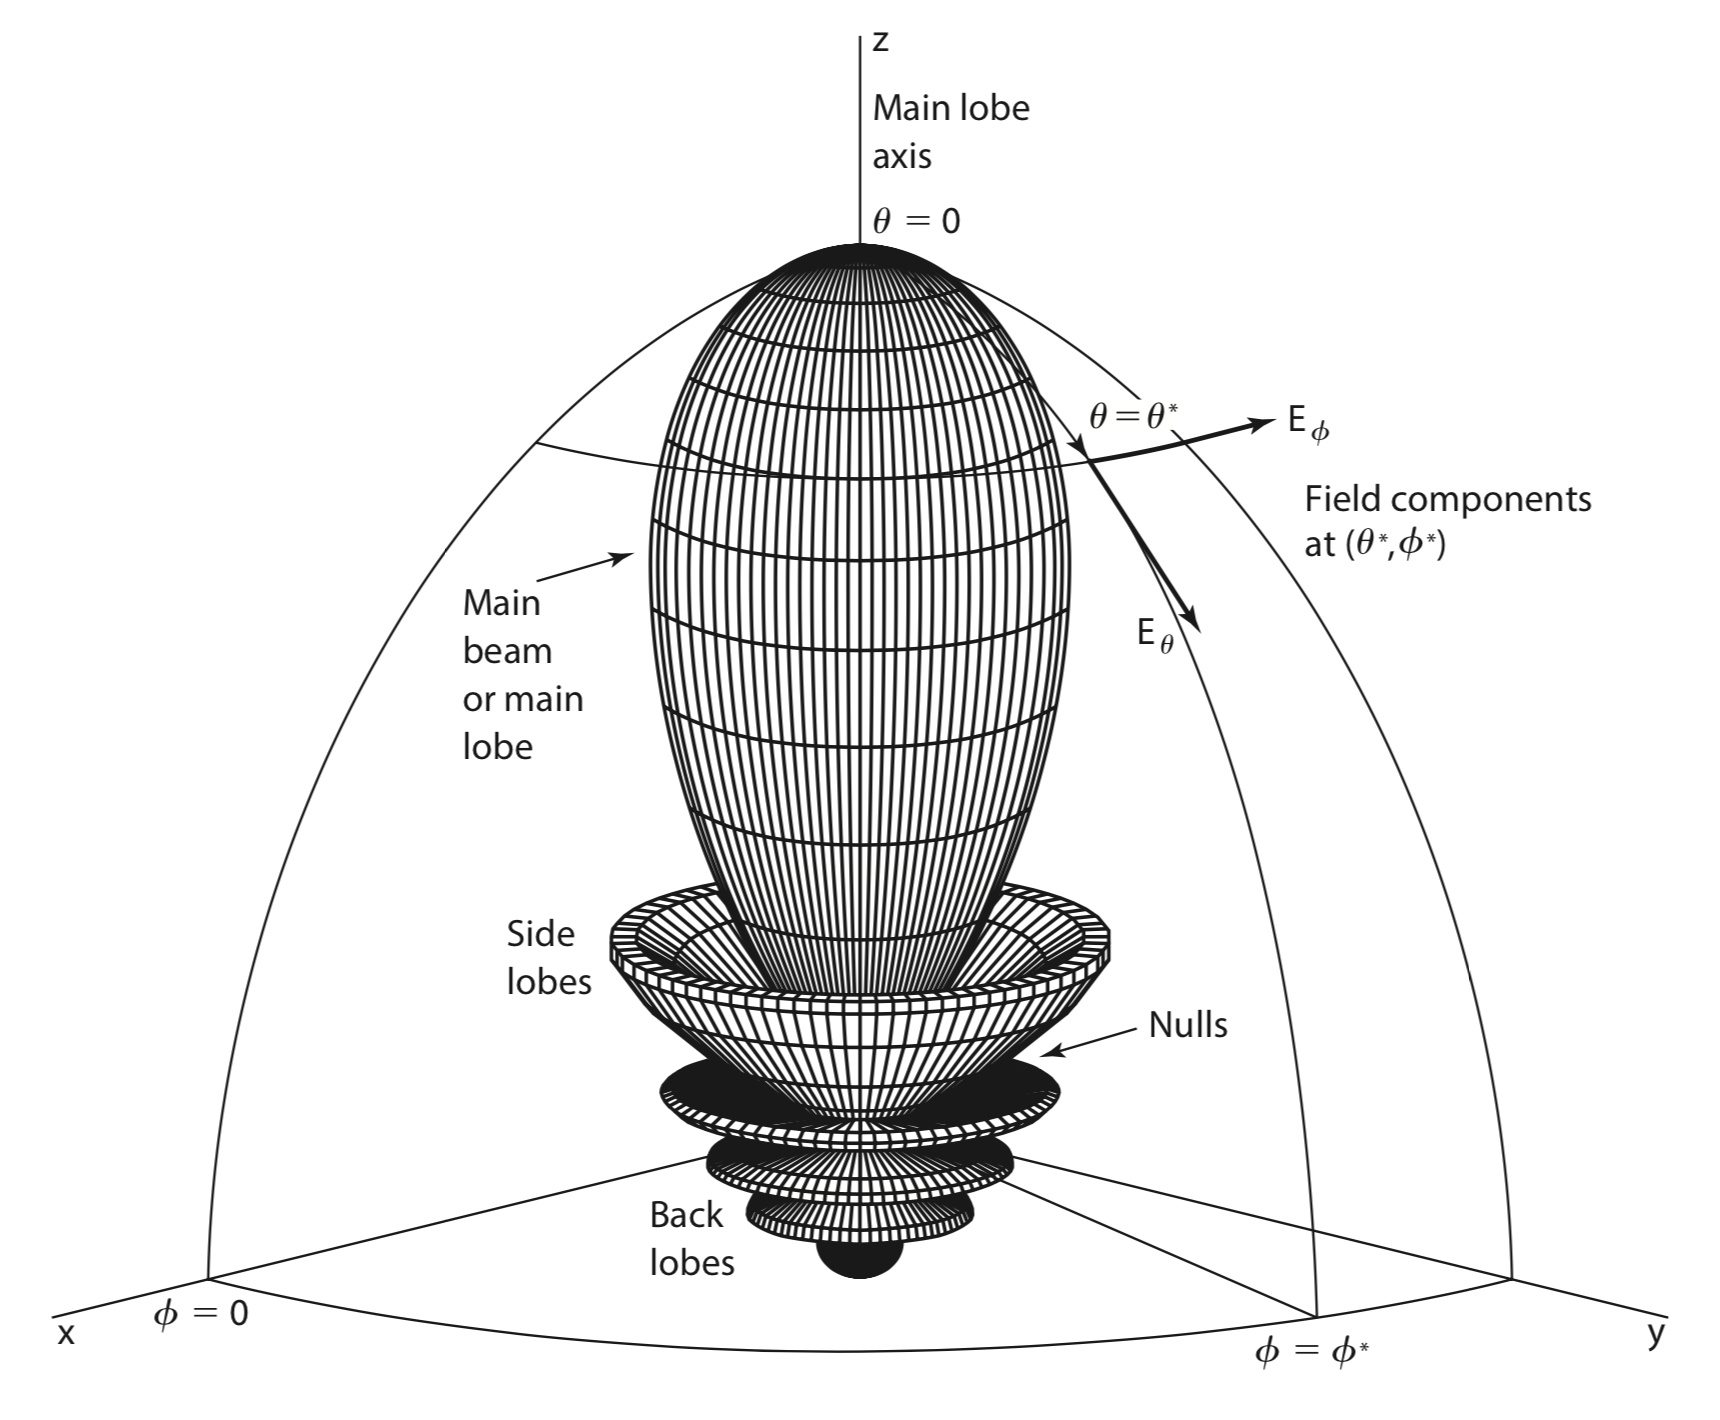
\includegraphics[width=0.8\linewidth]{../figures/diag_rad.png}
	\caption{Diagramma di radiazione tridimensionale di un'antenna direzionale.\cite{cmb}}
	\label{diag_rad}
\end{figure}
    %%%%%%%%%%%%%%%%%%  CAPITOLO 1.3  %%%%%%%%%%%%%%%%%%%%

\section{Simulazione di sistemi ottici}\label{simulazioni}

\begin{figure}[!ht]
	\centering
	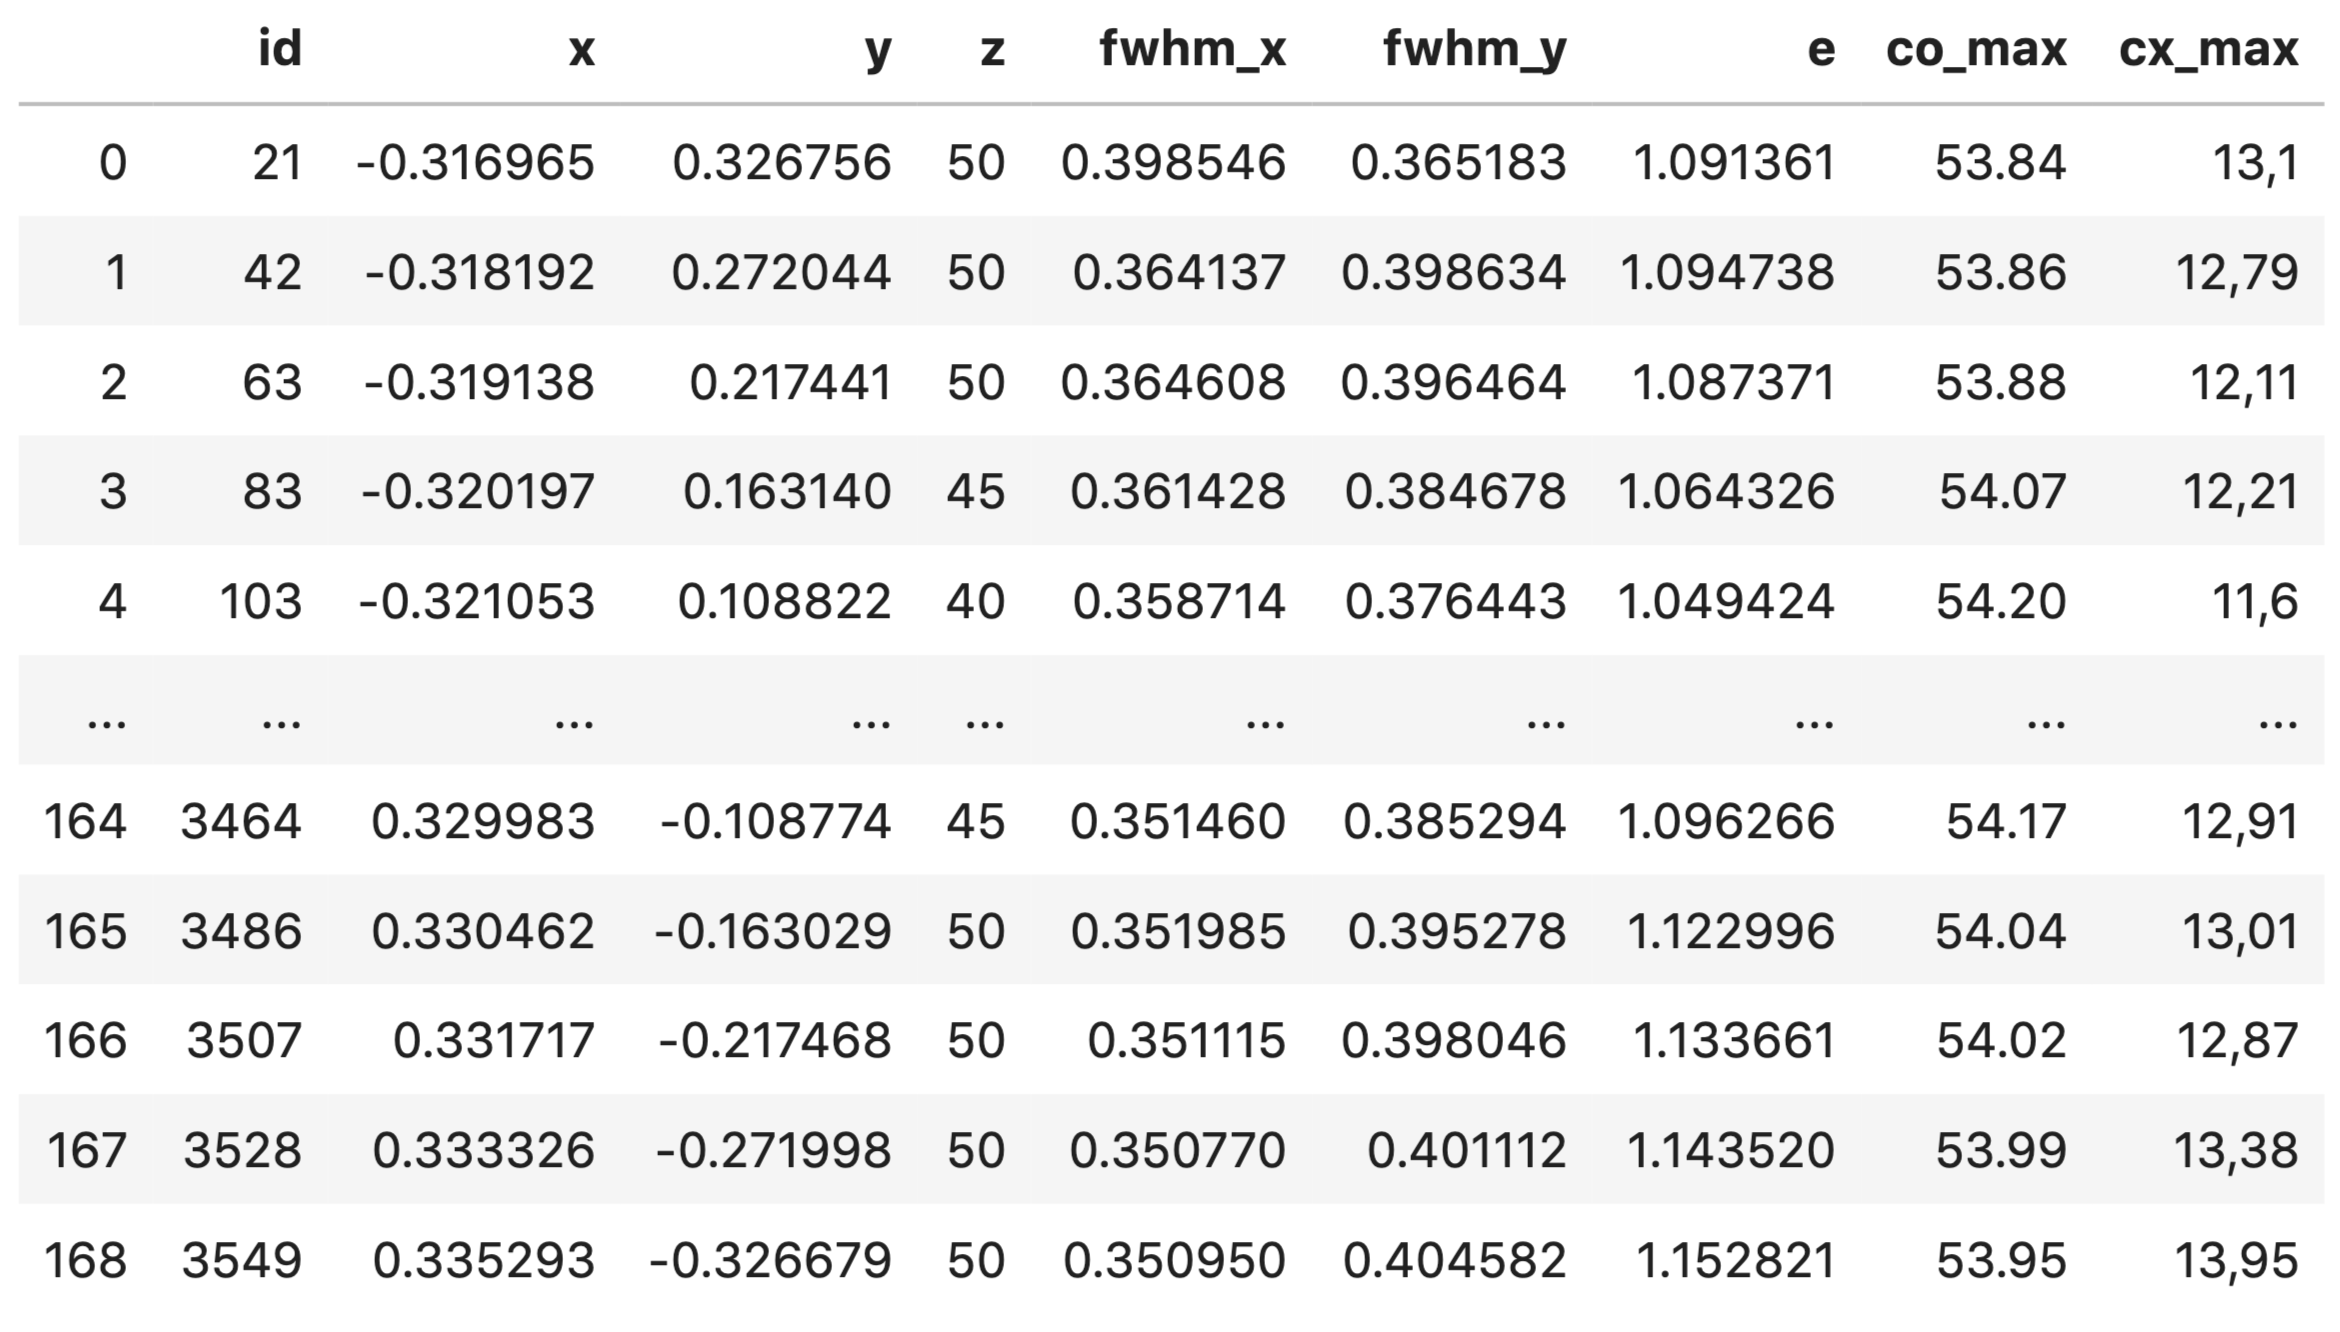
\includegraphics[width=\linewidth]{../figures/dataset.png}
	\caption{Dataset relativo allo strumento STRIP ottenuto tramite la simulazione in Grasp}
	\label{dataset}
\end{figure}

%%%%%%%%%%%%%%%%%%%%%%%%%%%%%%%%%%%%%%%%%%%%%%%%%%%%%%%
%%%%%%%%%%%%%%%%%%%%%%%%%%%%%%%%%%%%%%%%%%%%%%%%%%%%%%%
%%%%%%%%%%%%%%%%%%%%%%%%%%%%%%%%%%%%%%%%%%%%%%%%%%%%%%%
%                   FINE CAPITOLO 1                   %
%%%%%%%%%%%%%%%%%%%%%%%%%%%%%%%%%%%%%%%%%%%%%%%%%%%%%%%
%%%%%%%%%%%%%%%%%%%%%%%%%%%%%%%%%%%%%%%%%%%%%%%%%%%%%%%
%%%%%%%%%%%%%%%%%%%%%%%%%%%%%%%%%%%%%%%%%%%%%%%%%%%%%%%


%%%%%%%%%%%%%%%%%%%%  CAPITOLO 2  %%%%%%%%%%%%%%%%%%%%

\chapter{Regressione con reti neurali}\label{reg_nn}

	%%%%%%%%%%%%%%%%%%%  CAPITOLO 2.1  %%%%%%%%%%%%%%%%%%%

\section{Machine learning e tipi di rete}
Negli ultimi decenni il campo del \textit {machine learning} si è fortemente evoluto. È stata costruita un'ampia classe di algoritmi in grado di approssimare molto efficacemente processi non lineari. Tali architetture fanno parte di un particolare campo di ricerca, il \textit {Deep Learning}, che vede protagoniste le reti neurali artificiali. \\
Queste tecniche si basano su l'apprendimento tramite esempi, i quali sono rappresentati da coppie input-output come un'immagine e la sua descrizione (input: foto di un gatto, output: "gatto") o una posizione a cui è associato un particolare valore di campo elettrico (input: (x, y, z), output: E(x, y, z)). È quindi di fondamentale importanza avere a disposizione un ampio database attraverso il quale effettuare un \textit {training}. Le reti neurali consentono quindi di approssimare una corrispondenza, vera o presunta, tra un input e un output. 

	Esistono due classi di problemi affrontati con la tecnica delle reti neurali: la \textit {classificazione} e la \textit {regressione}.
La \textit {classificazione} individua l'appartenenza ad una classe e può essere supervisionata o non supervisionata. Parliamo di classificazione supervisionata quando sono note a priori le diverse classi di appartenenza; se invece si vogliono determinare delle classi di similitudine senza conoscere a priori i pattern rappresentativi, si ha un problema di classificazione non supervisionata. \\
Le reti neurali per la \textit {regressione} entrano in gioco quando, a partire da coppie input-output, si vuole determinare la funzione che approssimi al meglio la relazione.

	%%%%%%%%%%%%%%%%%%%  CAPITOLO 2.2  %%%%%%%%%%%%%%%%%%%

\section{Struttura di una rete neurale}
L'idea utopica su cui si fondano le reti neurali artificiali è quella di simulare il comportamenteo del cervello umano. Questo è un sistema estremamente complesso basato sull'interconnessioni di unità fondamentali: i \textbf {neuroni}. \\
Una rete neurale può essere schematizzata come in figura~\ref{schema_rete}.
\begin{figure}
	\centering
	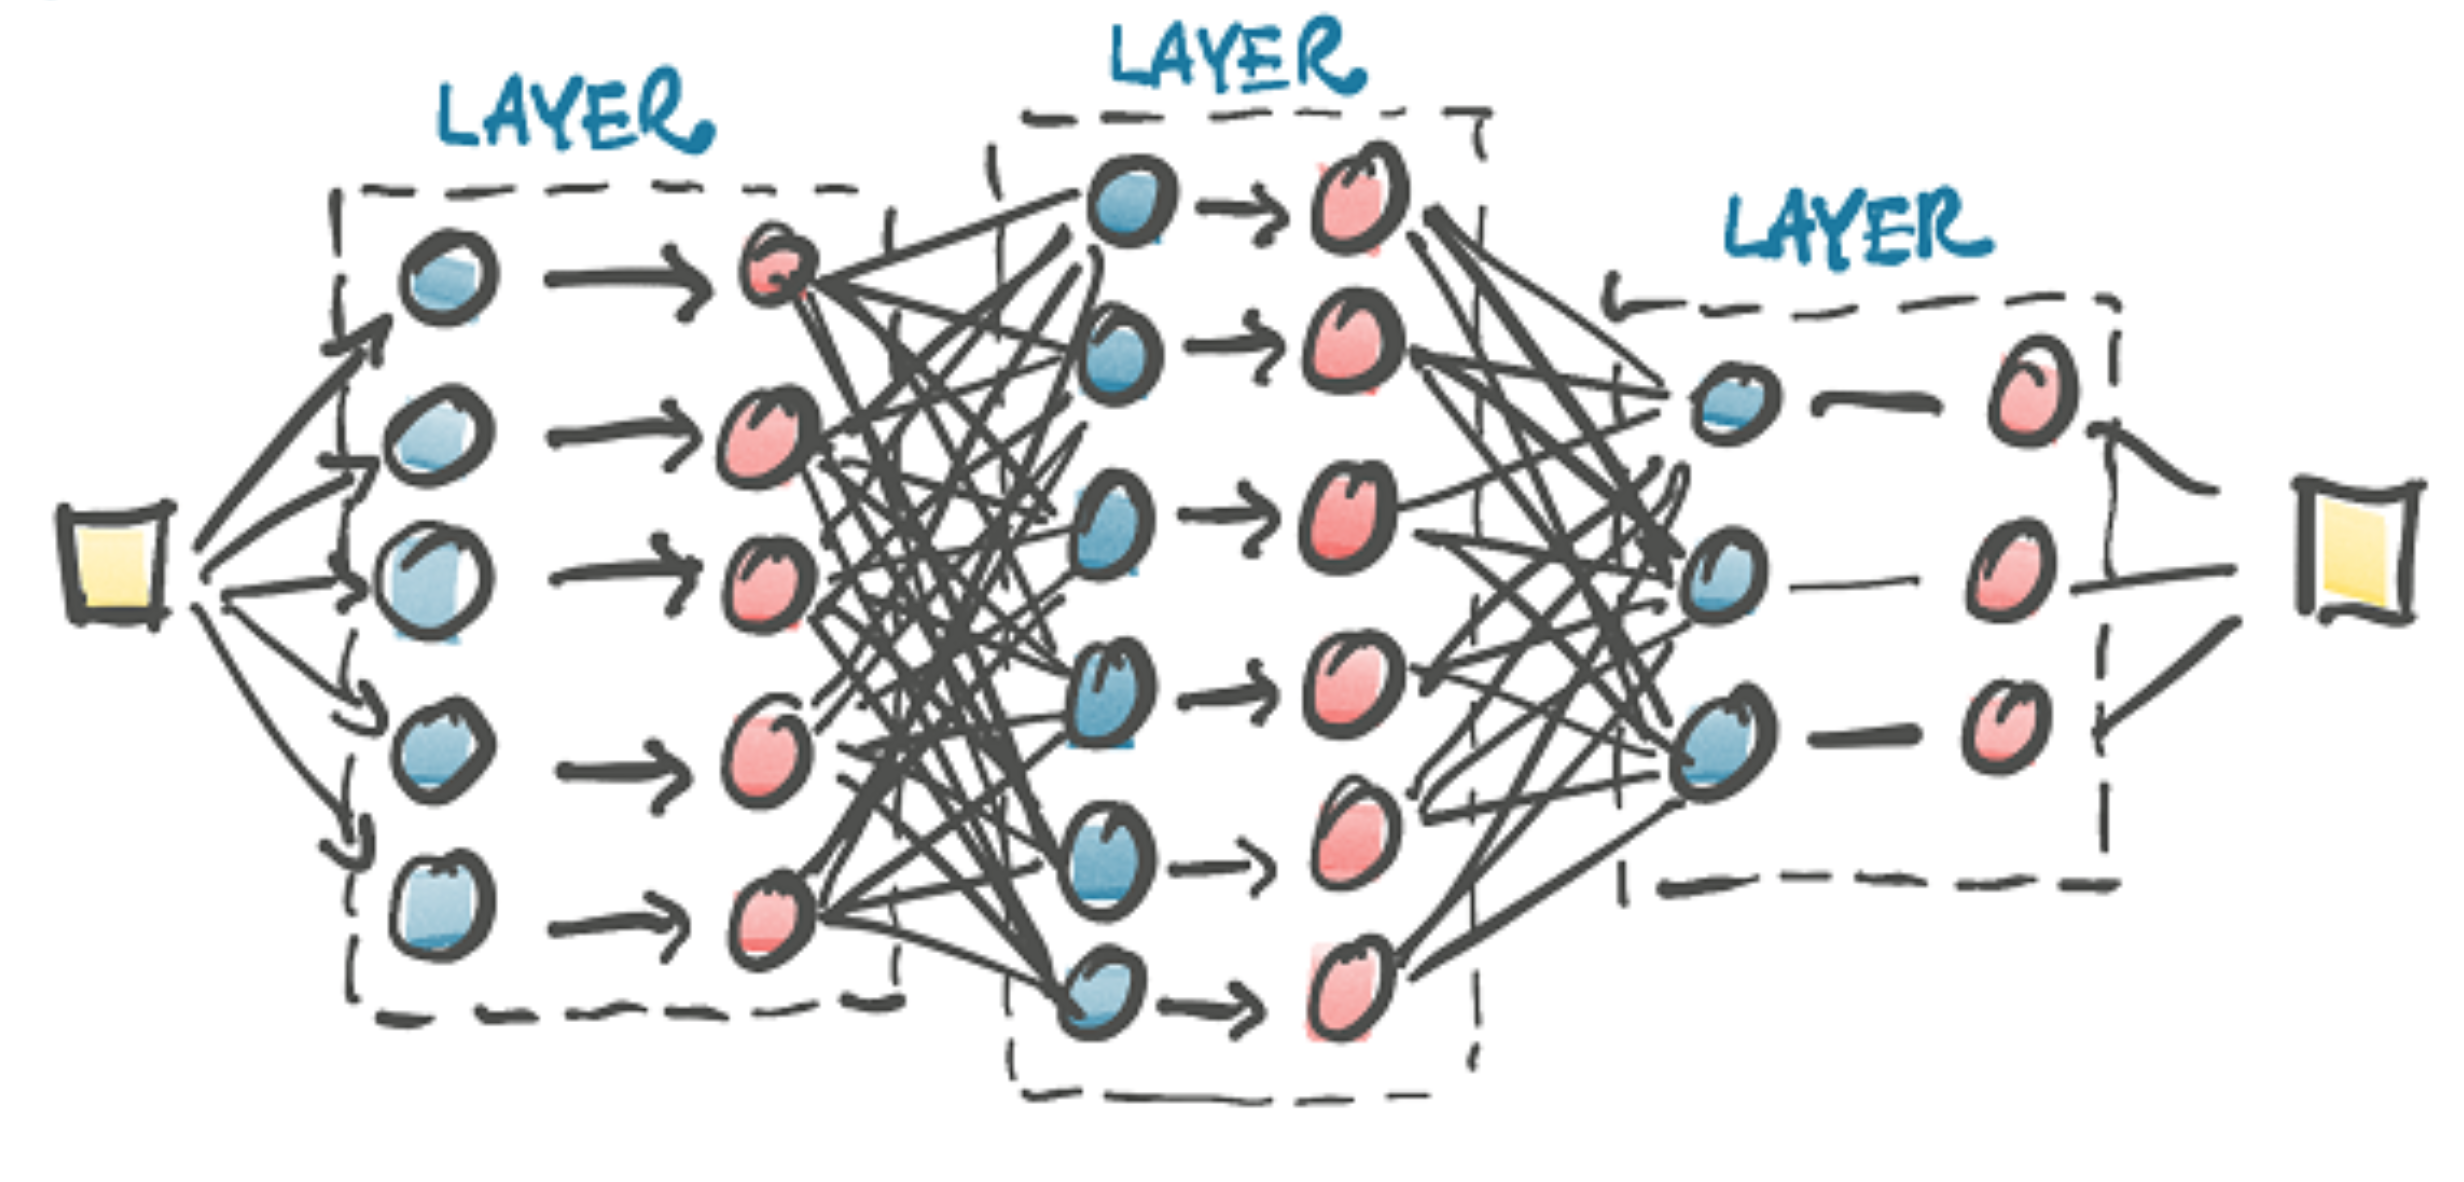
\includegraphics[scale=0.3]{../figures/schema_rete.jpg}
	\caption{Schema di una rete neurale con tre hidden layers\cite{stevens}}
	\label{schema_rete}
\end{figure}
Un insieme di neuroni che agiscono allo stesso livello è detto \textbf {layer} e l'interconnessione di diversi layers forma una rete.




%%%%%%%%%%%%%%%%%%%%%%%%%%%%%%%%%%%%%%%%%%%%%%%%%%%%%%%
%%%%%%%%%%%%%%%%%%%%%%%%%%%%%%%%%%%%%%%%%%%%%%%%%%%%%%%
%%%%%%%%%%%%%%%%%%%%%%%%%%%%%%%%%%%%%%%%%%%%%%%%%%%%%%%
%                   FINE CAPITOLO 2                   %
%%%%%%%%%%%%%%%%%%%%%%%%%%%%%%%%%%%%%%%%%%%%%%%%%%%%%%%
%%%%%%%%%%%%%%%%%%%%%%%%%%%%%%%%%%%%%%%%%%%%%%%%%%%%%%%
%%%%%%%%%%%%%%%%%%%%%%%%%%%%%%%%%%%%%%%%%%%%%%%%%%%%%%%


%%%%%%%%%%%%%%%%%%%%  CAPITOLO 3  %%%%%%%%%%%%%%%%%%%%

\chapter{Previsione delle proprietà di un diagramma di radiazione}\label{prev_param}
In questo capitolo varrà analizzato come sono stati previsti i parametri del diagramma di radiazione tramite i metodi di interpolazione e tramite l'utilizzo di reti neurali. \\
Nota: nei seguenti paragrafi verranno mostrati alcuni grafici rappresentativi dei risultati ottenuti. L'analisi è stata effettuata su ogni parametro di interesse ma i risultati qui riportati riguardano esclusivamente l'ellitticità. I risultati sono infatti molto simili al variare del parametro e quelli riportati sono grafici che hanno carattere generale. I parametri analizzati sono: ellitticità, FWHM (rispetto a x), FWHM (rispetto a y), componente co-polare massima e componente cross-polare massima.

    %%%%%%%%%%%%%%%%%%%  CAPITOLO 3.1  %%%%%%%%%%%%%%%%%%%

\section{Interpolazione}\label{interpolazione}
Per stimare le proprietà di un diagramma di radiazione attraverso strumenti classici di interpolaizione ho utilizzato due metodi: \texttt{interp2d} del modulo \texttt{scipy.interpolate}, basato su un'interpolazione lineare, e \texttt{curve fit} del modulo \texttt{scipy.optimize}, che ha permesso di fittare i dati attraverso un paraboloide.
Per poter effettuare l'interpolazione dei parametri e in seguito verificare la sua bontà, il dataset in fig.~\ref{dataset} è stato suddiviso in due subsets, considerando righe alterne, che ho chiamato \texttt{data\_int} e \texttt{data\_check}. Così facendo è stato possibile utilizzare metà dei dati per l'interpolazione e l'altra metà per la valutazione dell'errore tra il parametro stimato e quello esatto.

         %%%%%%%%%%%%%%%%%%%  CAPITOLO 3.1.1  %%%%%%%%%%%%%%%%%%%

\subsection{Interp2d}\label{interp2d}
\begin{figure}[t]
	\centering
	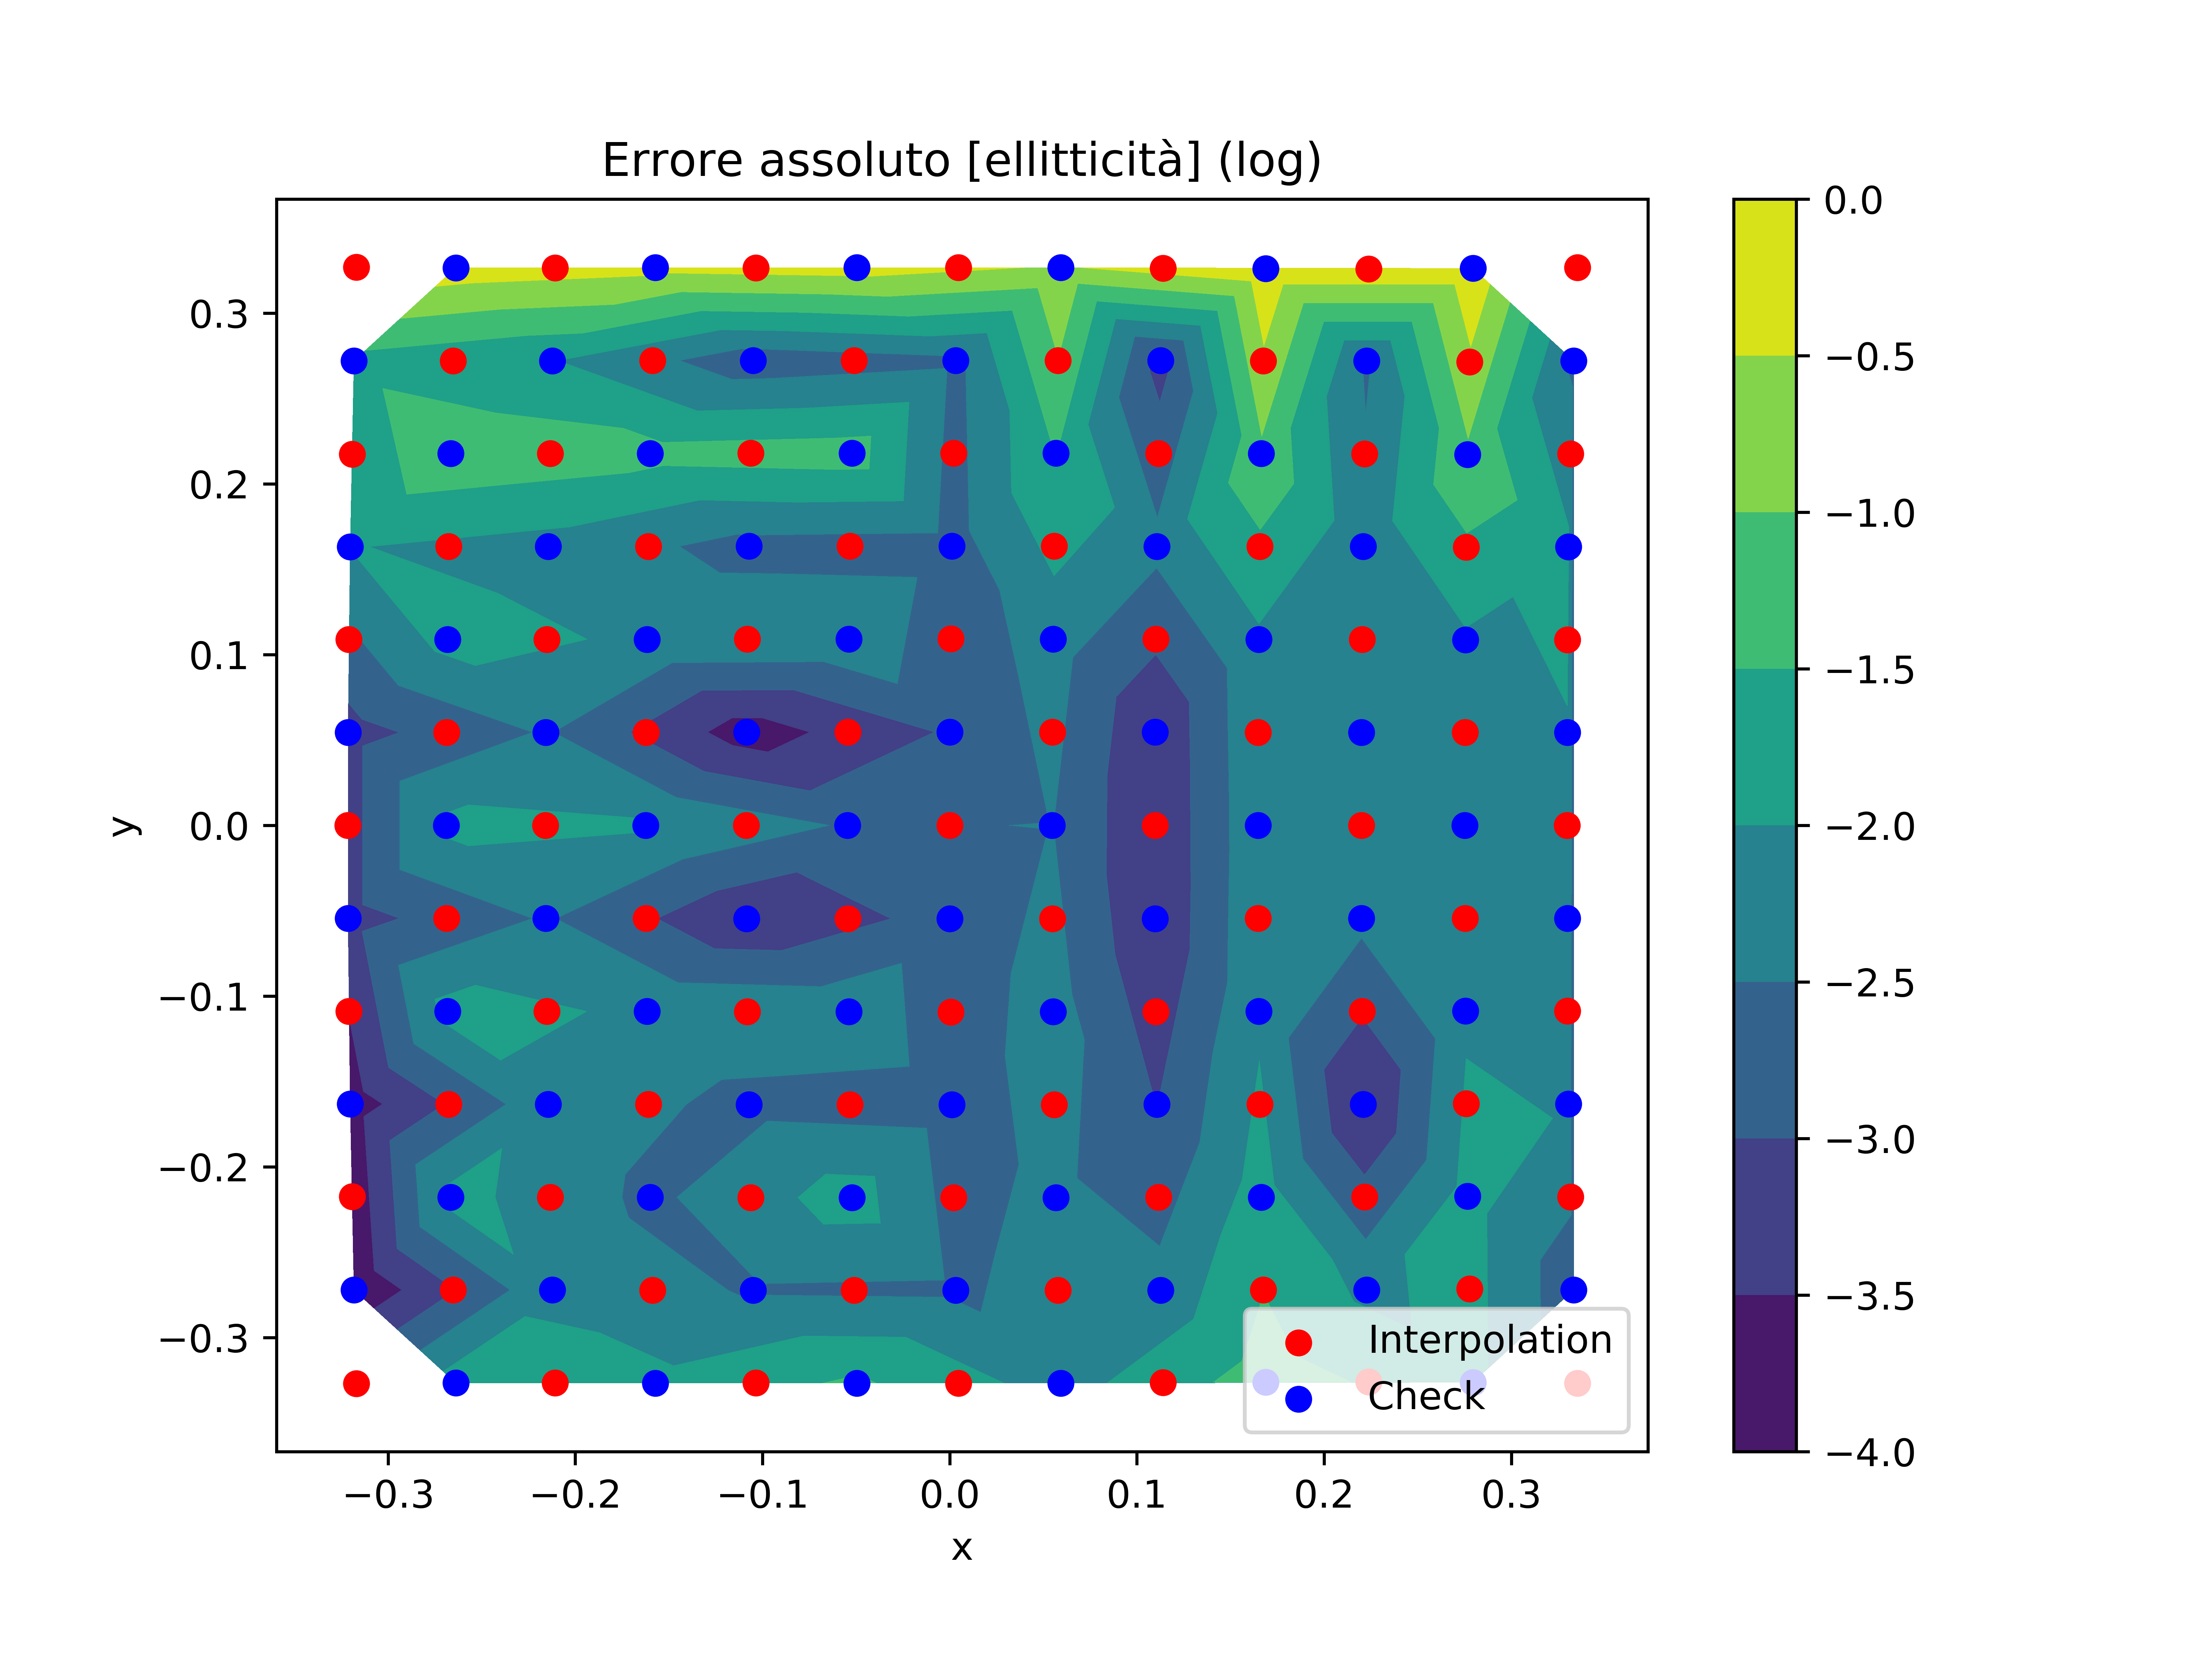
\includegraphics[scale=0.8]{../figures/errore_assoluto_ell.png}
	\caption{Contour plot in scala logaritmica dell'errore assoluto tra ellitticità interpolata tramite il metodo \texttt{interp2d} e ellitticità corretta. In rosso sono evidenziati i punti attraverso i quali è stata effettuata l'interpolazione mentre in blu sono rappresentati i punti nei quali è stato valutato l'errore.}
	\label{err_interp2d}
\end{figure}
Il metodo \texttt{interp2d} effettua l'interpolazione a partire da una griglia bidimensionale\footnote{La griglia non deve essere necessariamente regolare.}, nel mio caso questa è rappresentata dalle coppie (x, y) appartenti al subset \texttt{data\_int}. Una volta specificato il parametro di interesse, l'algoritmo effettua un'interpolazione lineare e ritorna una funzione in grado di prevedere il valore del parametro in nuovi punti. \\
La successiva analisi ha riguardato la valutazione dell'errore tra il parametro stimato nei punti appartenenti a \texttt{data\_check} e il suo valore vero. In fig.~\ref{err_interp2d} è mostrato l'errore assoluto relativo all'ellitticità.
Si nota che i punti della prima riga a partire dall'alto sono quelli affetti da errore massimo e, come verrà specificato nella sez.~\ref{risultati_interpolazione}, tali anomalie di bordo hanno determinato la scelta del metodo \texttt{curve fit} come termine di paragone con le reti neurali.

         %%%%%%%%%%%%%%%%%%%  CAPITOLO 3.1.2  %%%%%%%%%%%%%%%%%%%

\subsection{Curve Fit}\label{curve_fit}
Il metodo \texttt{curve\_fit} permette di fittare i dati con una funzione non lineare tramite il metodo dei minimi quadrati. Il metodo restituisce i valori ottimali dei parametri \texttt{popt} che minimizzano la discrepanza \texttt{f(xdata, *popt) - ydata}\footnote{In particolare \texttt{xdata} è una coppia (x, y) e \texttt{ydata} è il valore del parametro di interesse.}. Anche in questo caso ho utilizzato i due subset, \texttt{data\_int} e \texttt{data\_check}, per effettuare rispettivamente la regressione e la valutazione dell'errore. Nel mio caso il fit è stato eseguito su un paraboloide in quanto questo richiama la forma della superficie focale. \\
\begin{figure}
	\centering
	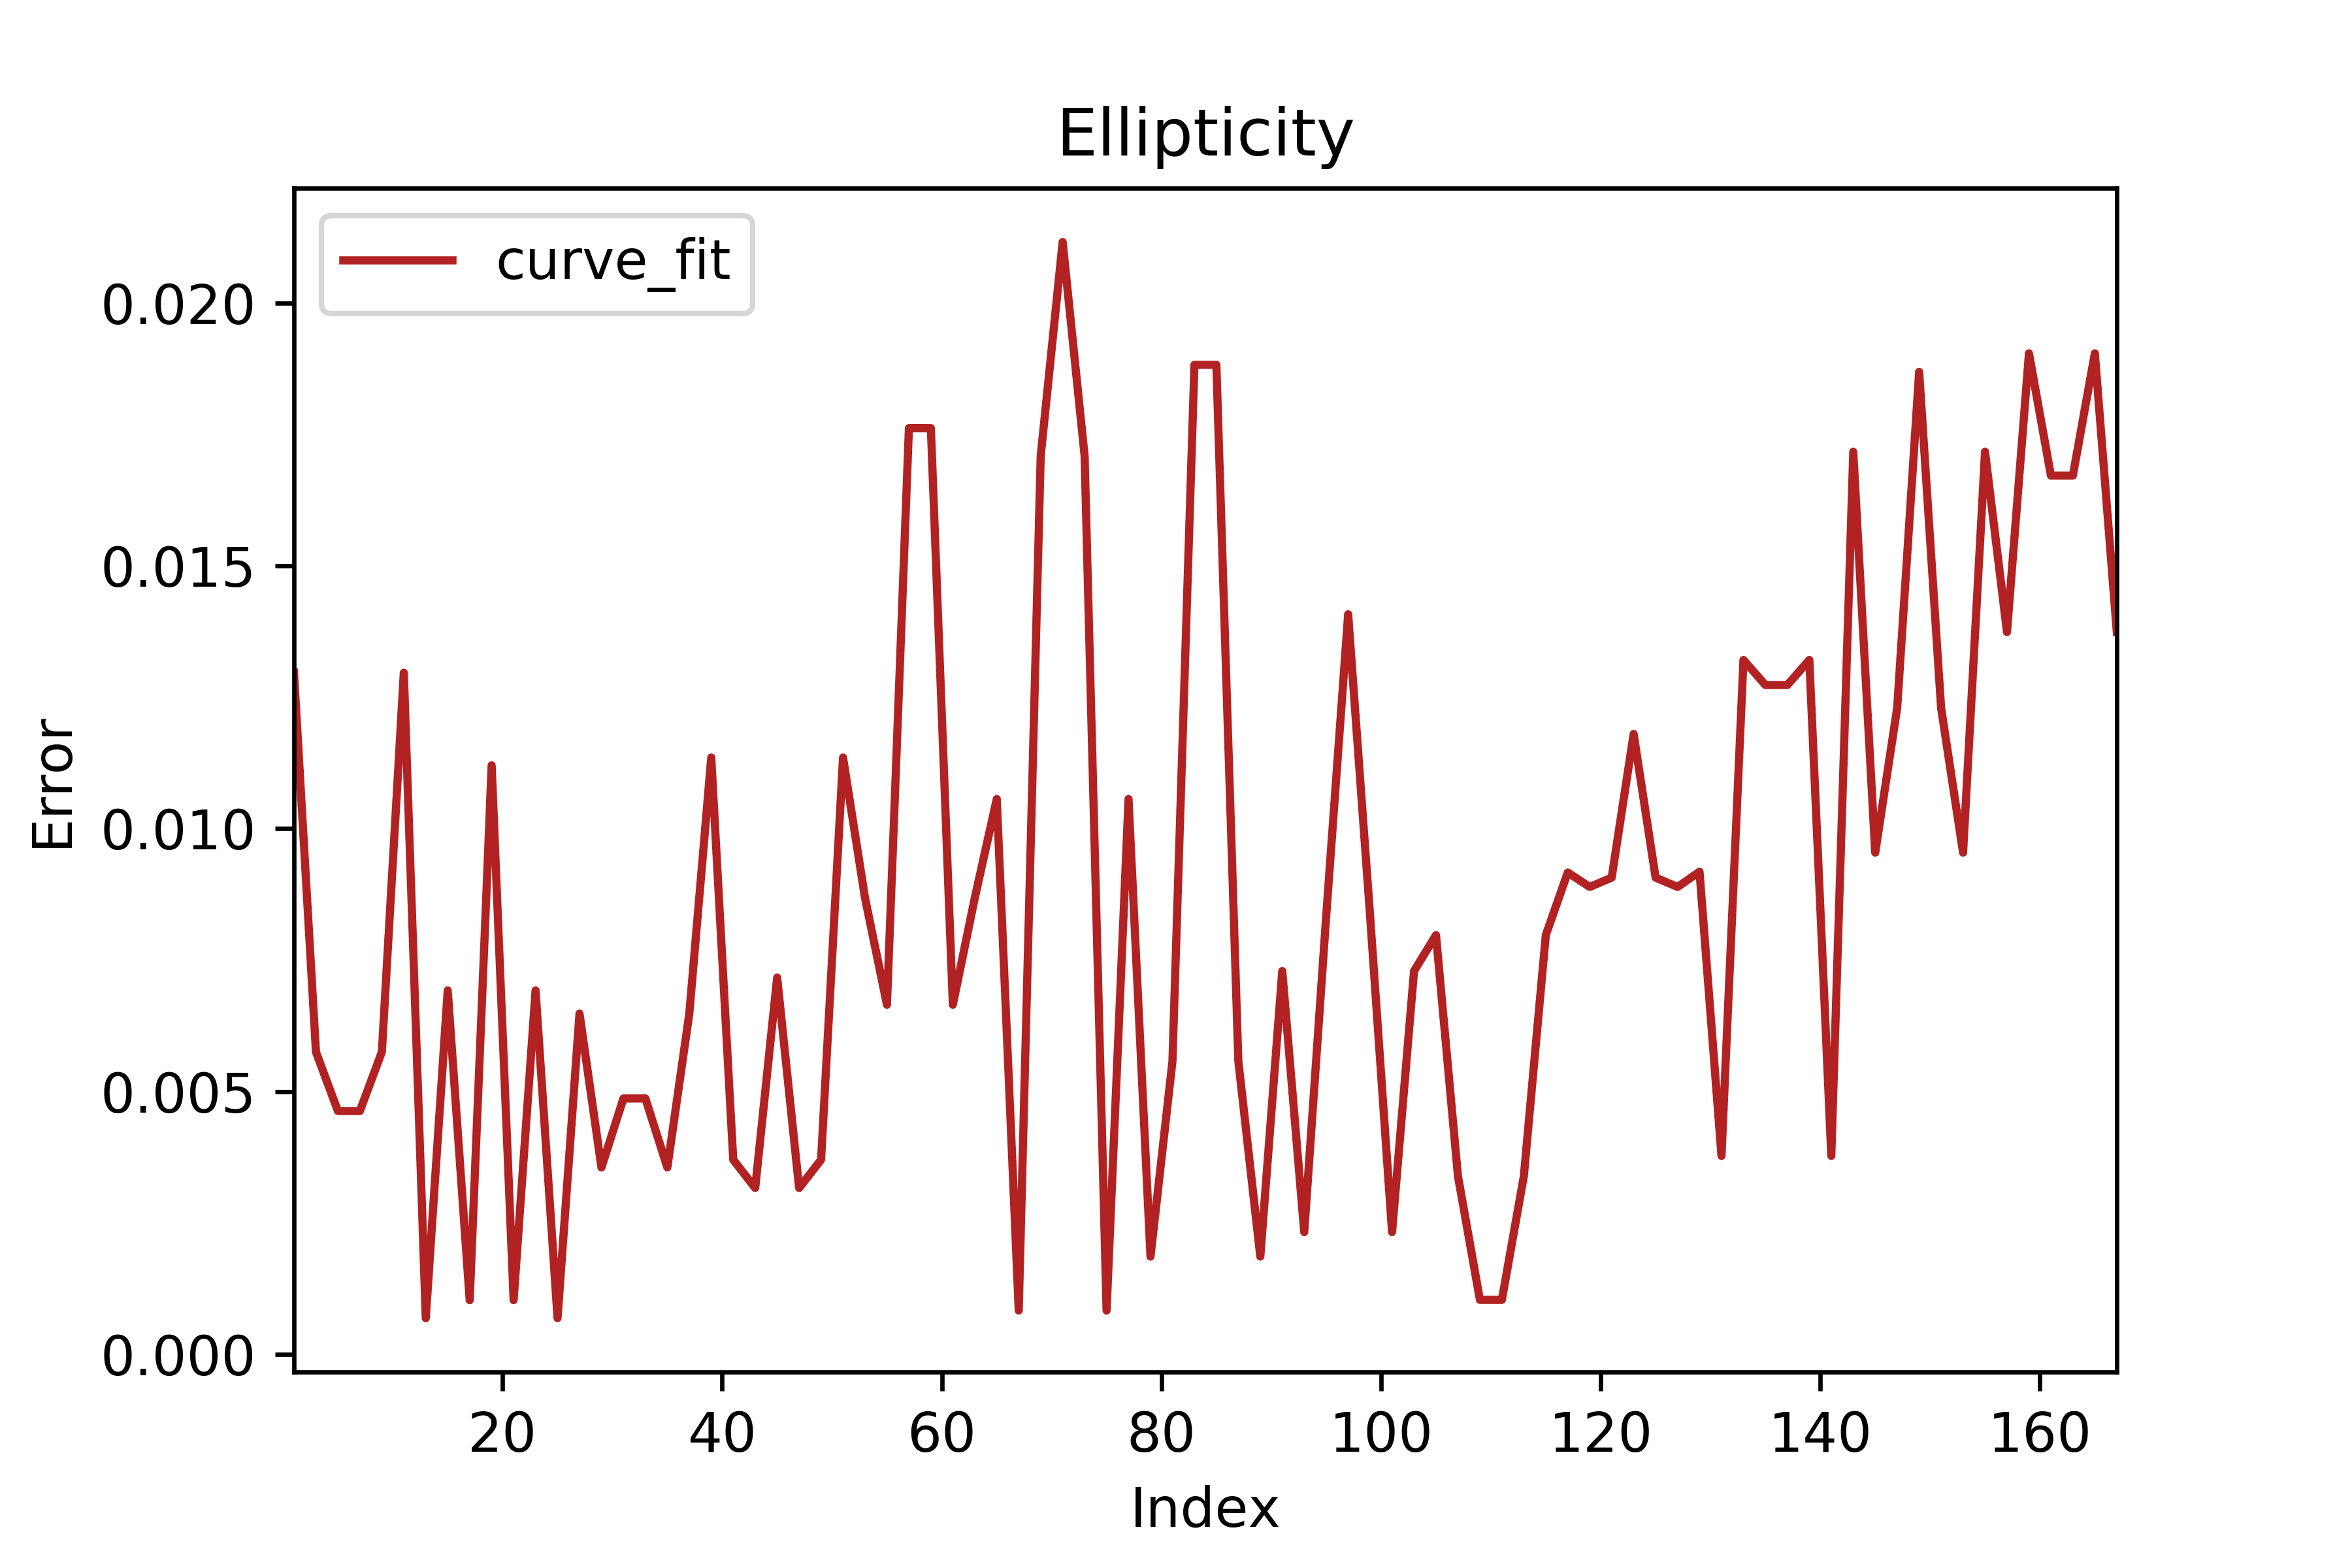
\includegraphics[scale=0.8]{../figures/error_curve_fit.png}
	\caption{Plot dell'errore assoluto tra ellitticità interpolata tramite il metodo \texttt{curve\_fit} e ellitticità corretta.}
	\label{err_curve_fit}
\end{figure}

        %%%%%%%%%%%%%%%%%%%  CAPITOLO 3.1.3  %%%%%%%%%%%%%%%%%%%

\subsection{Risultati dell'interpolazione}\label{risultati_interpolazione}
In fig.~\ref{err_int} sono confrontate le curve che rappresentano l'errore tra dato interpolato e dato corretto per i due metodi utilizzati. Si nota immediatamente la presenza di alcuni punti problematici riguardanti \texttt{interp2d} che non rendono possibile un confronto tra le due curve.
\begin{figure}[!ht]
	\centering
	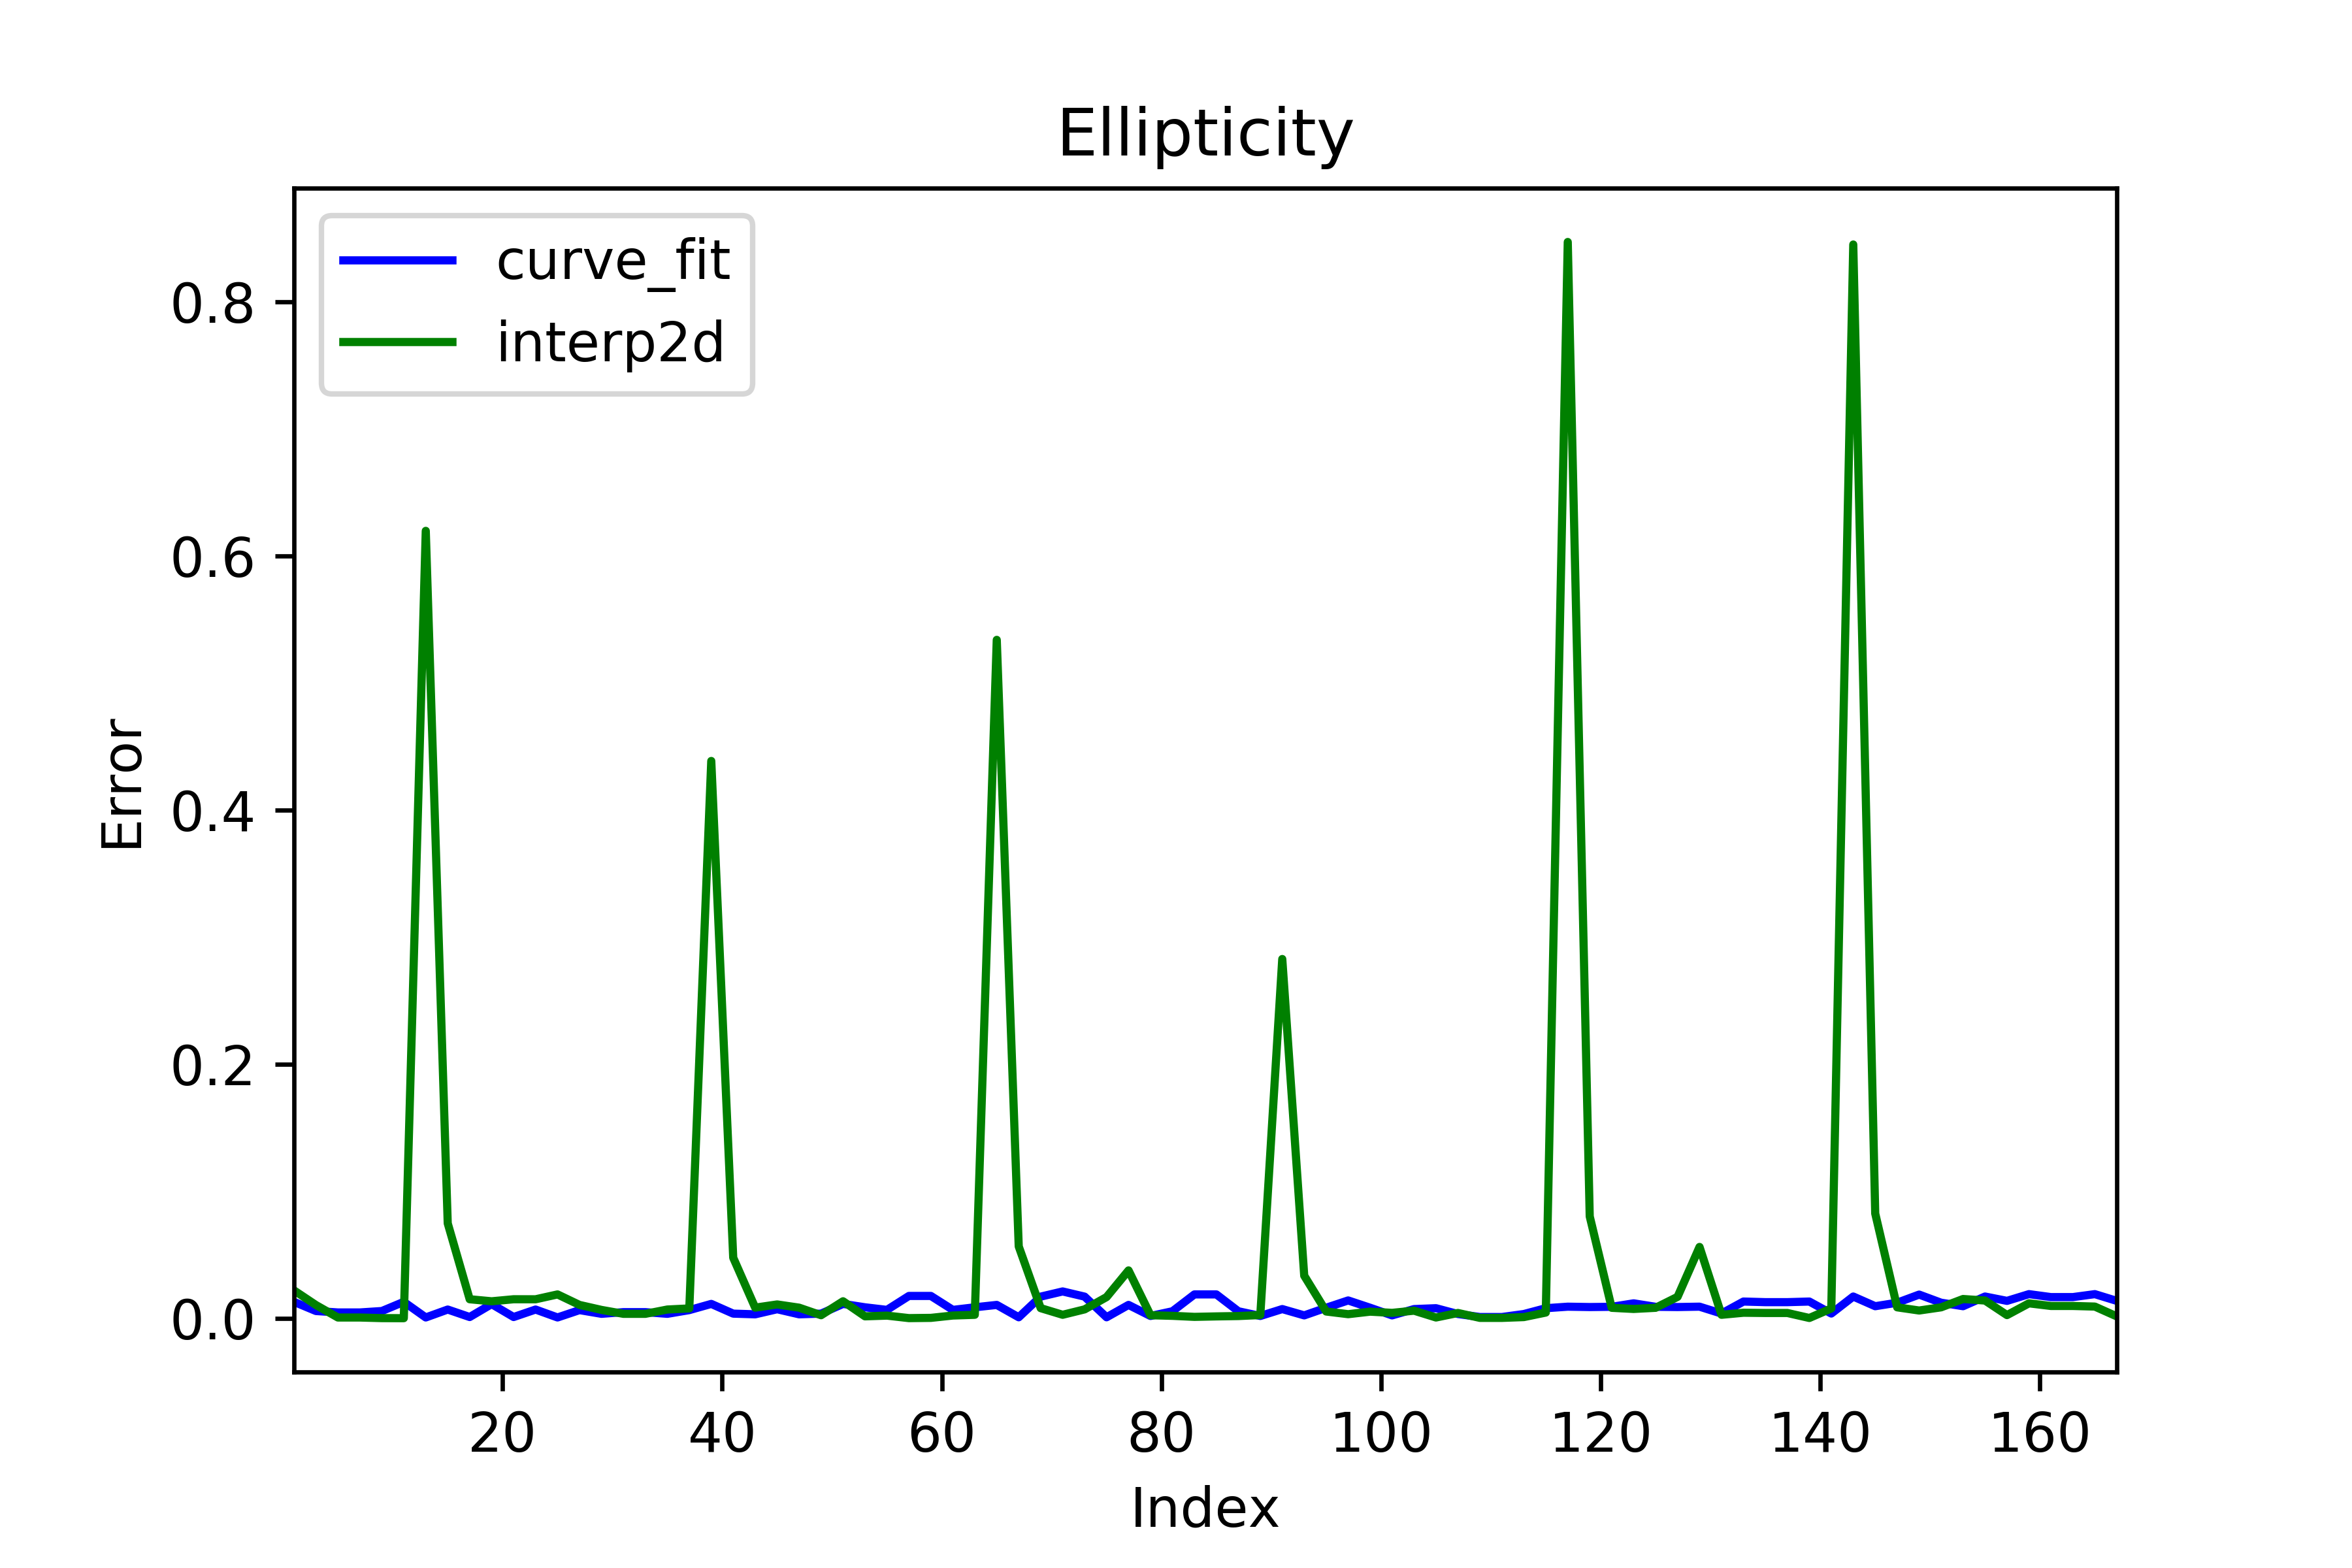
\includegraphics[scale=0.8]{../figures/error_comparison_all.png}
	\caption{Confronto dell'errore relativo ai due metodi di interpolazione.}
	\label{err_int}
\end{figure}

Analizzando più in dettaglio il comportamento del metodo \texttt{interp2d} è possibile mostrare che i punti affetti da errore maggiore sono punti di bordo. L'analisi è stata fatta plottando il valore interpolato e valore esatto del parametro per ogni riga di punti della griglia 13x13.
In fig.~\ref{plot_row} è mostrato il diverso comportamento di \texttt{interp2d} per una riga di punti di bordo e una riga di punti interni alla griglia.

\begin{figure}[!ht]
\centering
	\begin{subfigure}{0.8\textwidth}
	    \centering
	    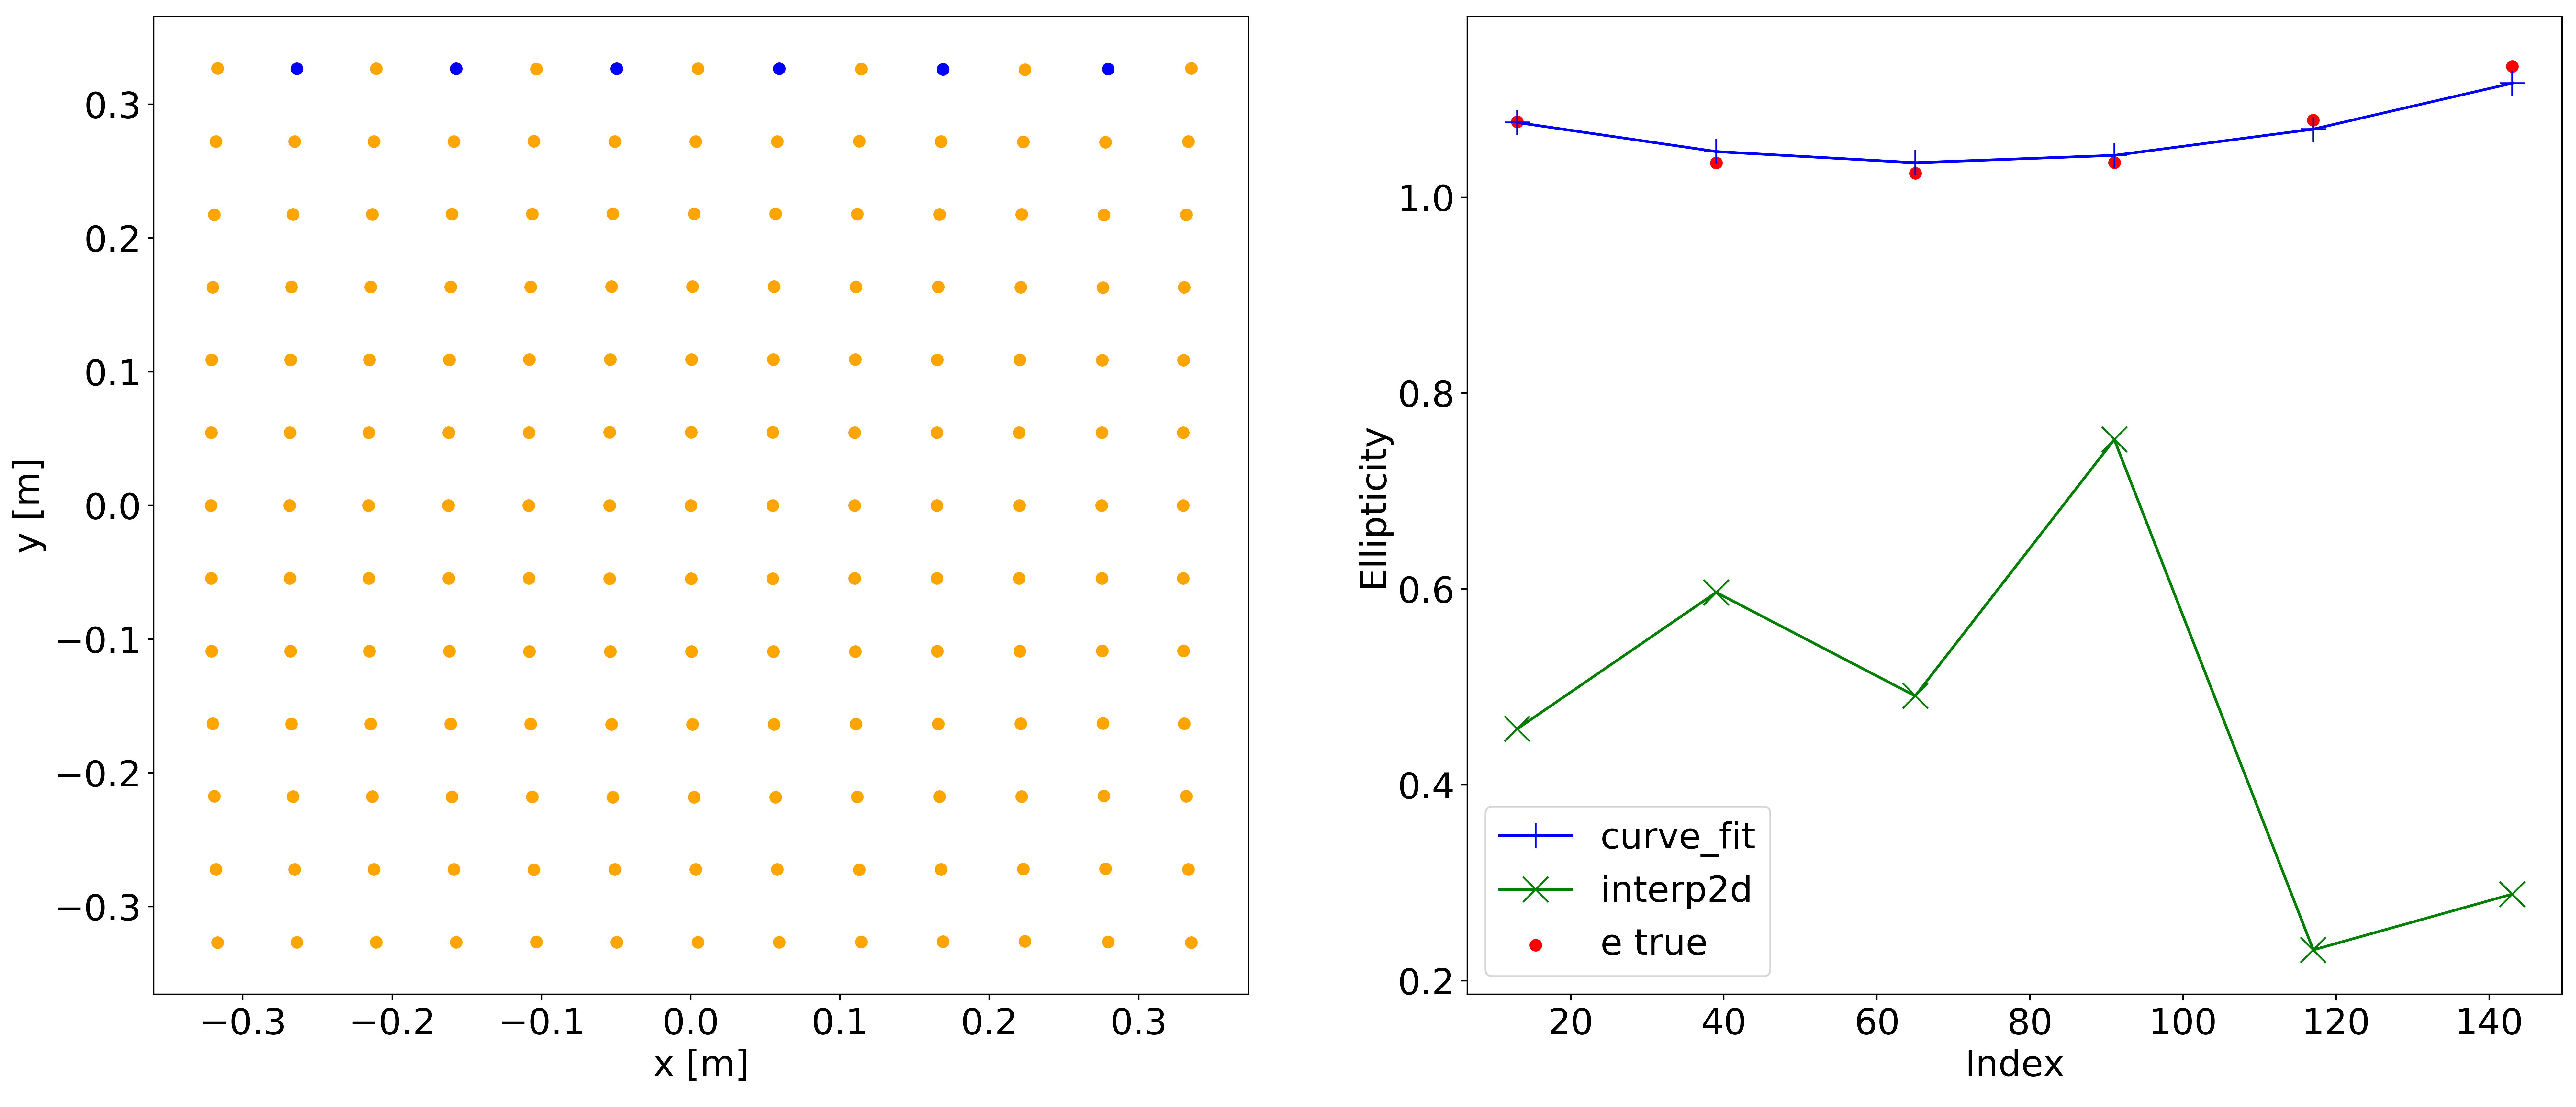
\includegraphics[width=0.8\linewidth]{../figures/row_bordo.png}
	    \caption{Punti di bordo}
	    \label{plot_row_bordo}
	\end{subfigure}
\newline
	\begin{subfigure}{0.8\textwidth}
		\centering
	    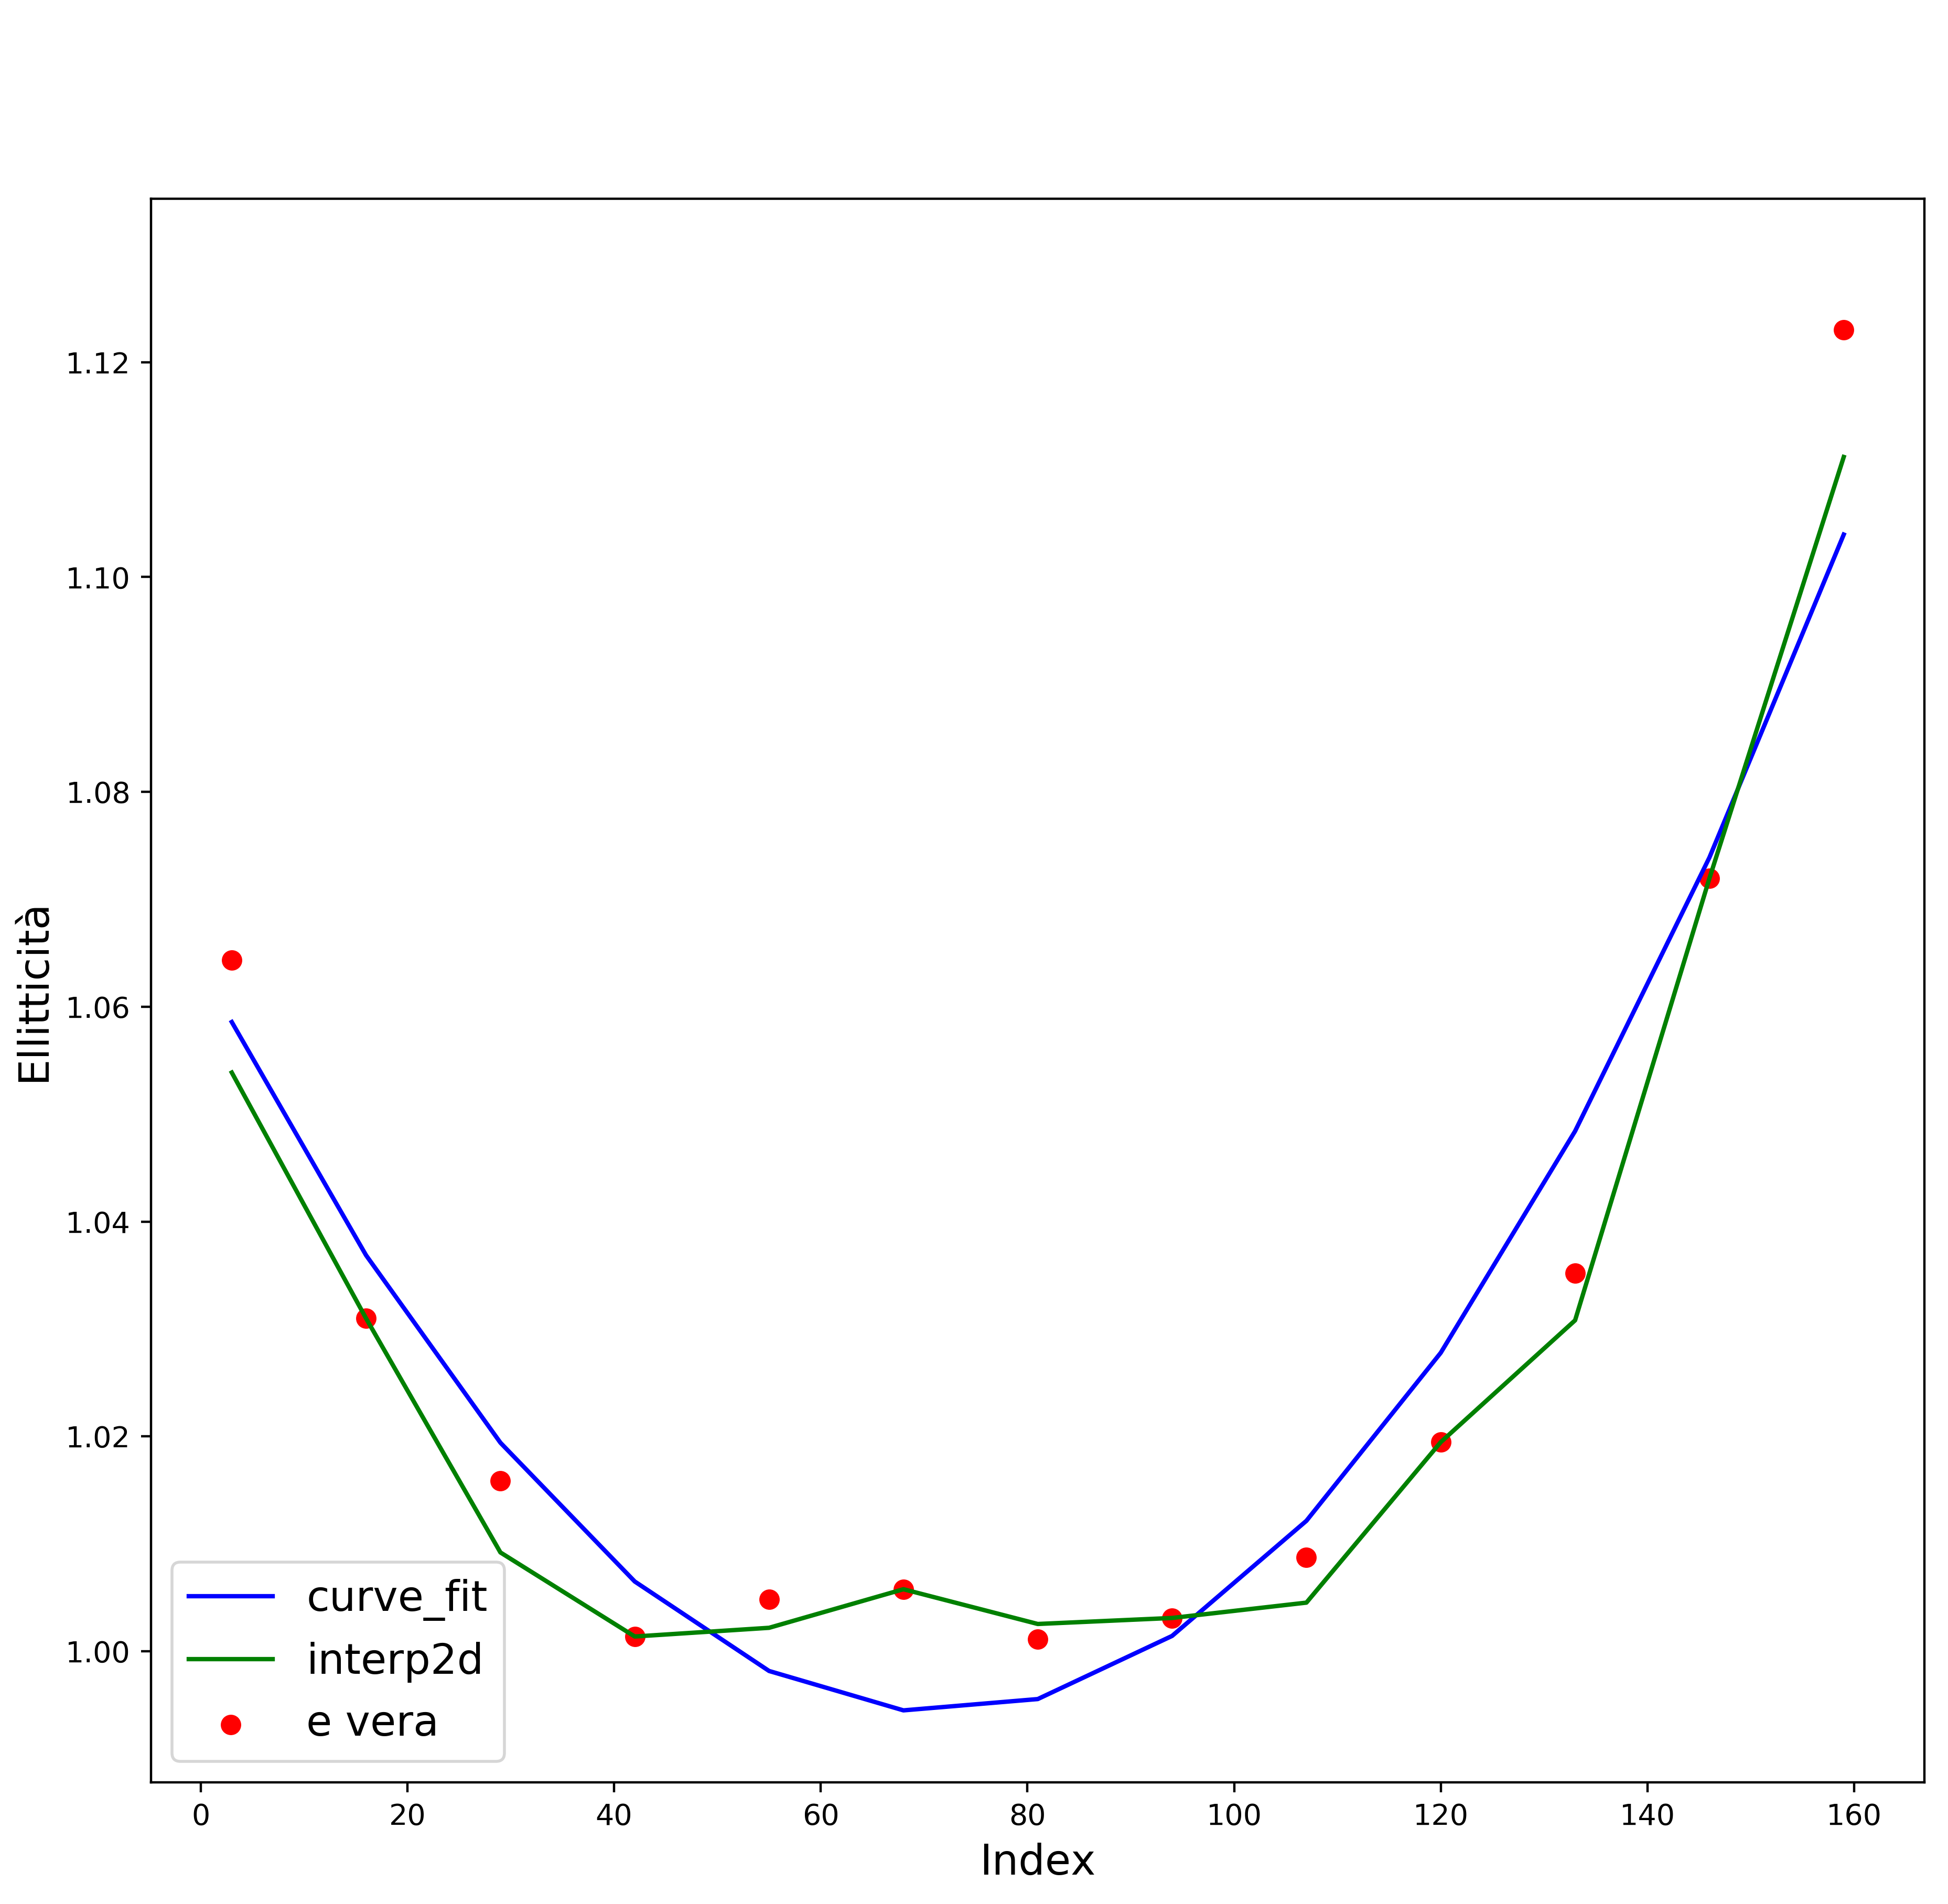
\includegraphics[width=0.8\linewidth]{../figures/row_interno.png}
		\caption{Punti interni}
		\label{plot_row_interno}
	\end{subfigure}
\caption{Plot del valore dell'ellitticità per due diverse righe di punti. Nel grafico~\ref{plot_row_bordo} è mostrato l'andamento dell'ellitticità per una riga di punti di bordo mentre nel grafico~\ref{plot_row_interno} viene analizzata l'ellitticità di una riga interna della griglia di punti.}
\label{plot_row}
\end{figure}

Per poter andare a confrontare gli errori dei due metodi di interpolazione ho creato un subset del dataset iniziale rimuovendo i punti più esterni: \texttt{data\_mask}. Il passaggio successivo è stato plottare novamente l'errore come in fig.~\ref{err_int} e il risultato ottenuto è mostrato in fig.~\ref{err_int_mask}.

\begin{figure}[!ht]
	\centering
	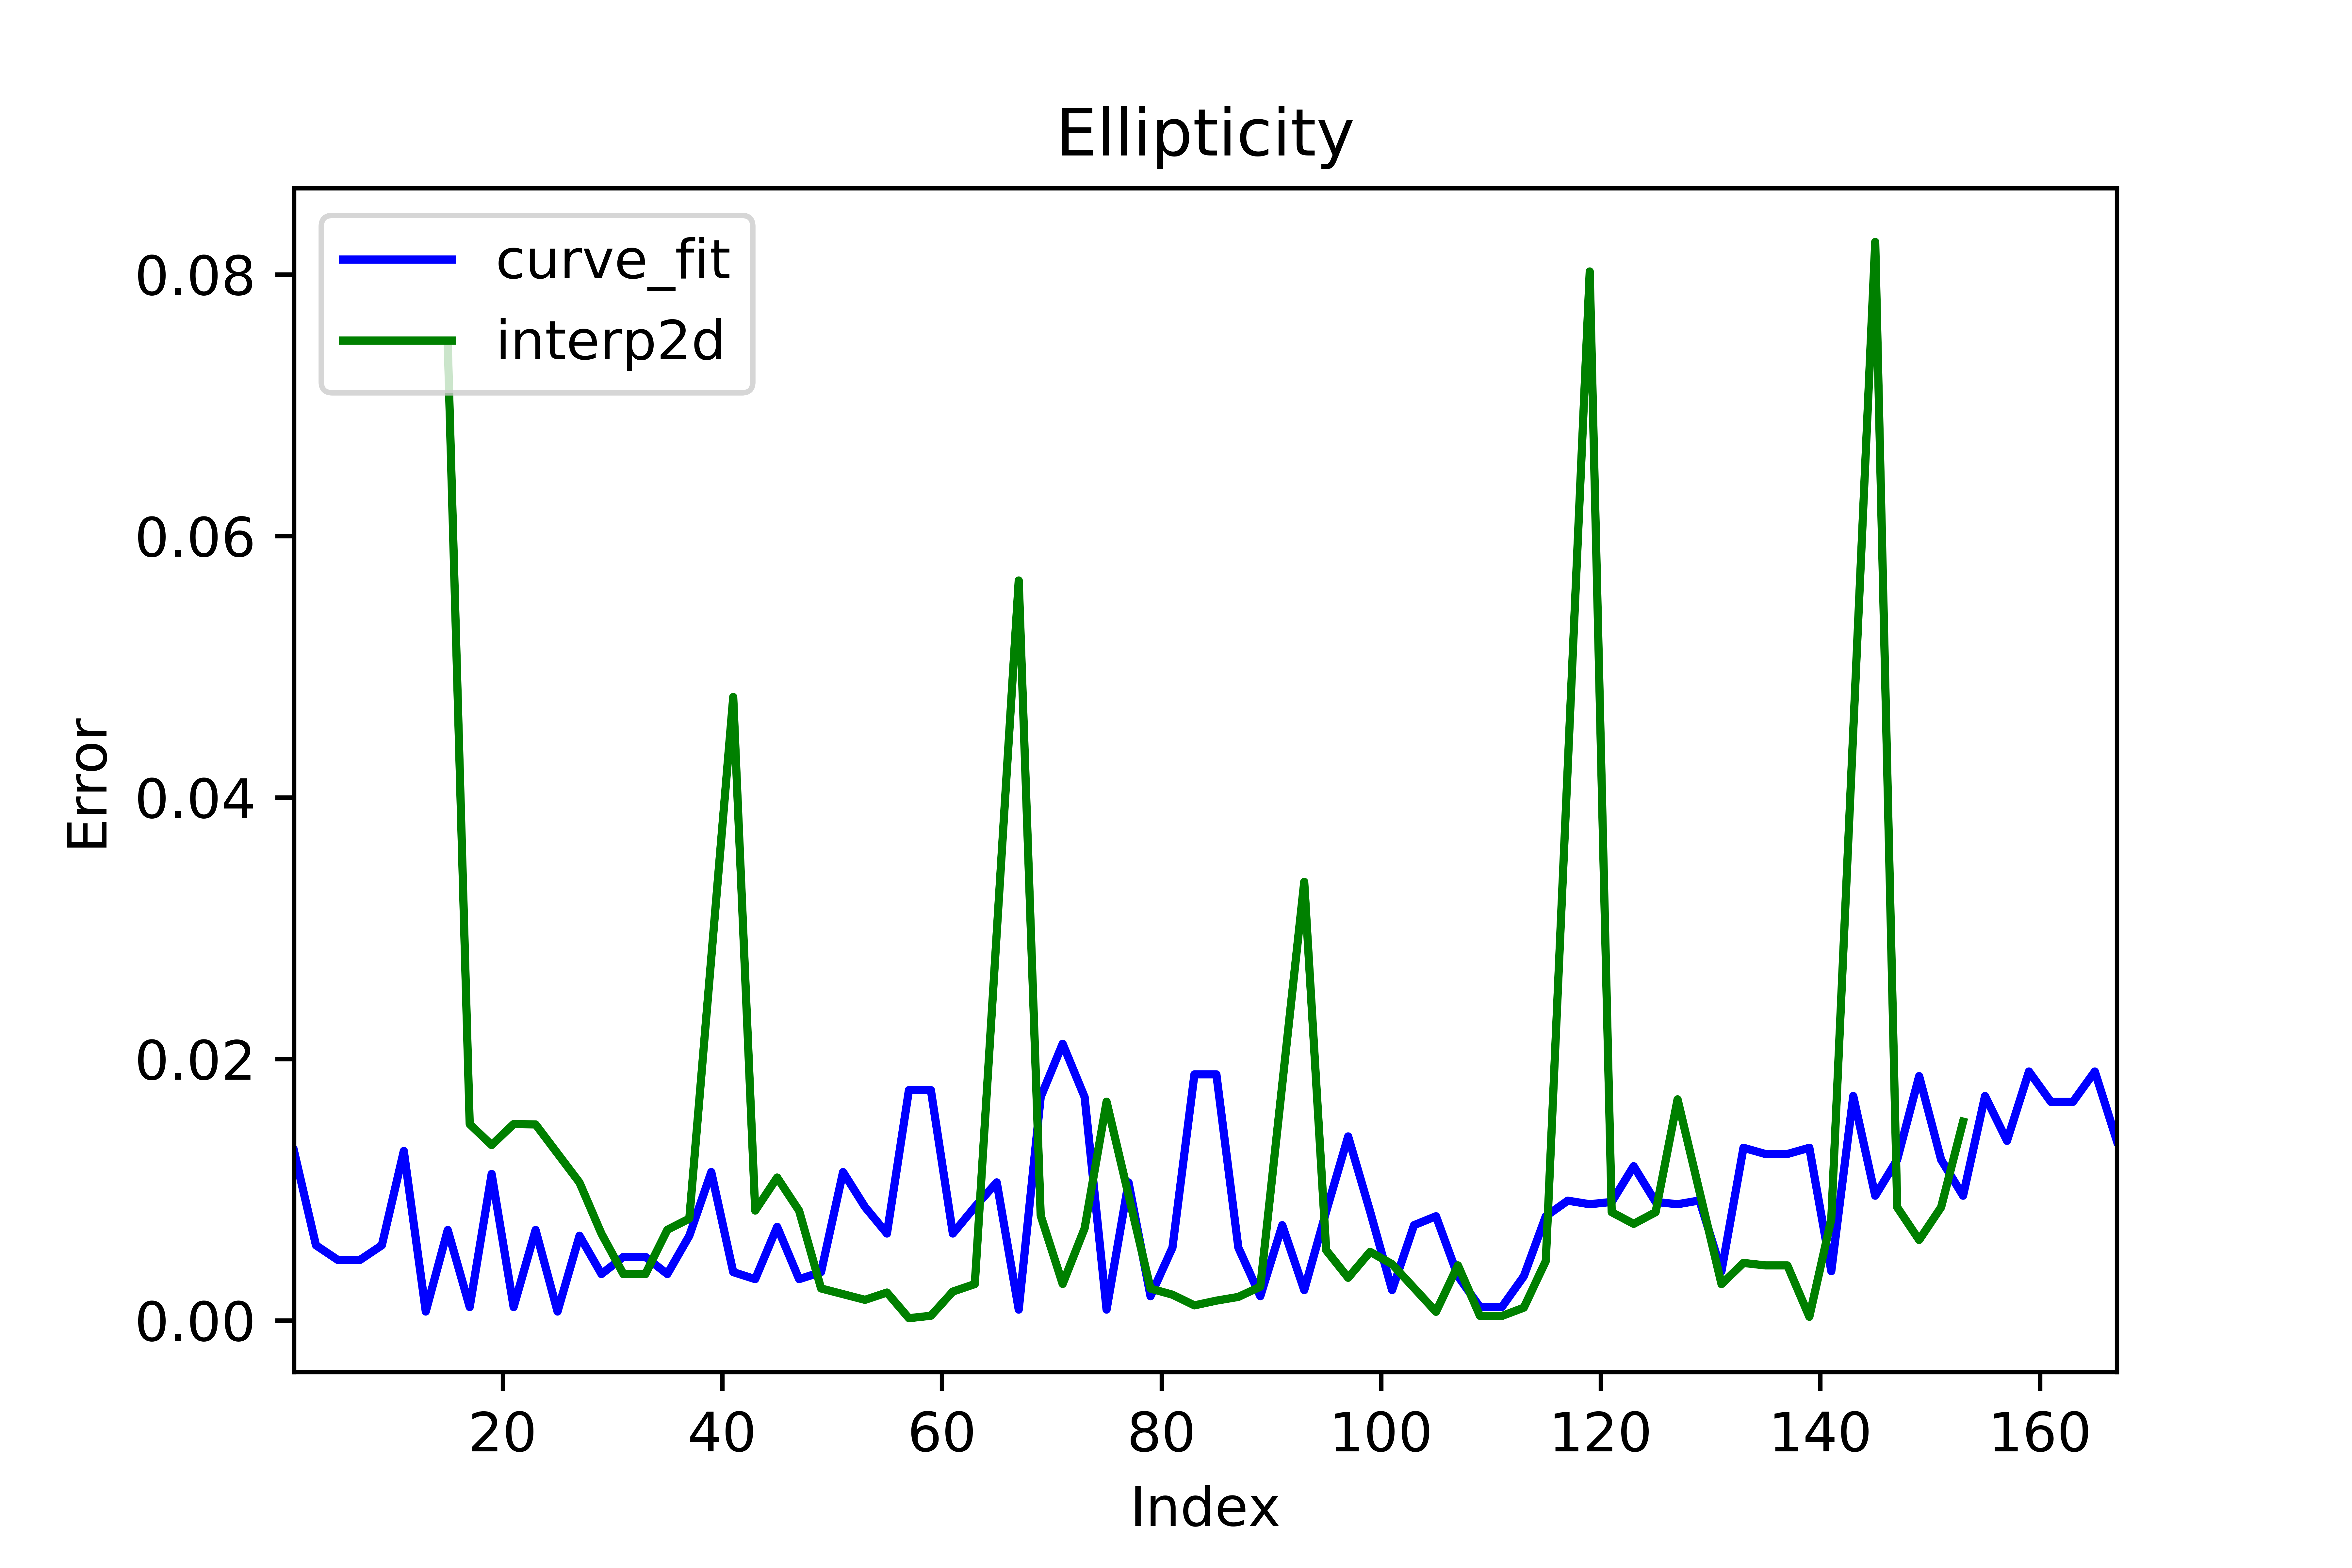
\includegraphics[scale=0.8]{../figures/error_comparison.png}
	\caption{Confronto dell'errore relativo ai due metodi di interpolazione dopo aver rimosso i punti di bordo.}
	\label{err_int_mask}
\end{figure}

Il plot in fig.~\ref{err_int_mask} mostra ancora dei punti nei quali l'errore di \texttt{interp2d} è molto maggiore rispetto a quello di \texttt{curve\_fit}, per tale motivo ho deciso di considerare esclusivamente il metodo \texttt{curve\_fit} come termine di paragone tra i risultati relativi all'interpolazione e quelli relativi alle reti neurali, come verrà mostrato nella sezione~\ref{risultati}.


     %%%%%%%%%%%%%%%%%%%  CAPITOLO 3.2  %%%%%%%%%%%%%%%%%%%
\section{Reti neurali}\label{reti_neurali}
In questa sezione mostro come sono state create le architetture delle reti neurali utilizzati per effettuare la regressione, come sono stati gestiti i dati a disposizione per definire \texttt{training set} e \texttt{validazion set} e com'è avvenuto il processo di training. Infine verrà presentato il confronto dei risultati ottenuti tramite l'utilizzo dell'interpolazione e della rete neurale (~\ref{risultati}).

        %%%%%%%%%%%%%%%%%%%  CAPITOLO 3.2.1  %%%%%%%%%%%%%%%%%%%

\subsection{Architettura della rete}\label{architettura}
Quando si costruisce una rete neurale è necessario definire alcuni elementi che andranno a caratterizzare una particolare architettura di rete.
Tali elementi sono:
\begin{itemize}
	\item La dimensione dell'\textit{input layer}.
	\item La dimensione dell'\textit{output layer}.
	\item Il numero di \textit{hidden layers}.
	\item Il numero di \textit{neuroni} per ogni hidden layer.
	\item La \textit{funzione di attivazione}.
	\item L'\textit{optimizer}.
	\item La \textit{loss function}.
\end{itemize}

La scelta dei loro valori non è mai univoca, non esiste una regola fissa per avere la ricetta perfetta che porta ai risultati migliori.
Nel mio lavoro di tesi ho utilizzato 6 diverse architetture; alcuni degli elementi appena citati sono stati mantenuti invariati per ogni architettura, mentre altri sono stati variati. \\
\noindent Per poter decrivere al meglio la scelta delle architetture è necessario fare alcune osservazioni. \\
\noindent Uno dei problemi più diffusi nell'ambito delle reti neurali è quello dell'\textbf{overfitting}. Si va incontro ad overfitting quando, per esempio, si utilizza un numero estremamente elevato di neuroni se confrontato con gli elementi che si hanno a disposizione per il training.
Ogni neurone è infatti caratterizzato da due parametri liberi (\textit{weight} e \textit{bias}), la presenza di un elevato numero di parametri liberi fa si che la rete impari perfettamente la corrispondenza tra input e output degli elementi nel training set, ma in tal modo si perde il carattere necessario per ottenere risultati validi. La dimensione del \textit{trainig set} andrà dunque a fissare un limite superiore del numero di neuroni totali della rete. \\
\noindent Un'ulteriore osservazione riguarda 

!!! nel mio caso non ho normalizzato i dati di input perchè la x e la y appartenevano già a dei "buoni" intervalli -> sono intorno all'unità

        %%%%%%%%%%%%%%%%%%%  CAPITOLO 3.2.2  %%%%%%%%%%%%%%%%%%%

\subsection{Pre Training}\label{pre_training}
Bla bla bla 

        %%%%%%%%%%%%%%%%%%%  CAPITOLO 3.2.3  %%%%%%%%%%%%%%%%%%%

\subsection{Training}\label{training}
Bla bla bla 

        %%%%%%%%%%%%%%%%%%%  CAPITOLO 3.2.4  %%%%%%%%%%%%%%%%%%%

\subsection{Confronto di risultati}\label{risultati}
Bla bla bla 

%%%%%%%%%%%%%%%%%%%%%%%%%%%%%%%%%%%%%%%%%%%%%%%%%%%%%%%
%%%%%%%%%%%%%%%%%%%%%%%%%%%%%%%%%%%%%%%%%%%%%%%%%%%%%%%
%%%%%%%%%%%%%%%%%%%%%%%%%%%%%%%%%%%%%%%%%%%%%%%%%%%%%%%
%                   FINE CAPITOLO 3                   %
%%%%%%%%%%%%%%%%%%%%%%%%%%%%%%%%%%%%%%%%%%%%%%%%%%%%%%%
%%%%%%%%%%%%%%%%%%%%%%%%%%%%%%%%%%%%%%%%%%%%%%%%%%%%%%%
%%%%%%%%%%%%%%%%%%%%%%%%%%%%%%%%%%%%%%%%%%%%%%%%%%%%%%%







%%%%%%%%%%%%%%%%%%%%  CAPITOLO 4  %%%%%%%%%%%%%%%%%%%%

\chapter{Conclusioni}\label{conclusioni}

%%%%%%%%%%%%%%%%%%%%%%%%%%%%%%%%%%%%%%%%%%%%%%%%%%%%%%%
%%%%%%%%%%%%%%%%%%%%%%%%%%%%%%%%%%%%%%%%%%%%%%%%%%%%%%%
%%%%%%%%%%%%%%%%%%%%%%%%%%%%%%%%%%%%%%%%%%%%%%%%%%%%%%%
%                   FINE CAPITOLO 4                   %
%%%%%%%%%%%%%%%%%%%%%%%%%%%%%%%%%%%%%%%%%%%%%%%%%%%%%%%
%%%%%%%%%%%%%%%%%%%%%%%%%%%%%%%%%%%%%%%%%%%%%%%%%%%%%%%
%%%%%%%%%%%%%%%%%%%%%%%%%%%%%%%%%%%%%%%%%%%%%%%%%%%%%%%


\bibliography{../bibliografia/my_bib}{}
\bibliographystyle{abbrv}


\end{document}








